% Appendix A

\chapter{Network Characterizations} % Main appendix title

\label{AppendixB} % For referencing this appendix elsewhere, use \ref{AppendixA}

\lhead{Appendix A. \emph{Appendix Title Here}} % This is for the header on each page - perhaps a shortened title

\section{Average Degree}

Degree $k_i$ is simply the number of edges connected to the node $i$. Average degree of a network $\langle k \rangle$ indicates the ratio of total number of edges, \textit{L}, to total number of nodes, \textit{N} in a graph.
 
\begin{equation}
\langle k \rangle = \frac{2L}{N}
\end{equation} 
 
In order not to count each link twice, the total number of edges is divided by $\frac{N}{2}$ instead of $N$. 
 

%\begin{figure}[htp]
%
%  \centering
%
% 
%
%    % Requires \usepackage{graphicx}
%
%    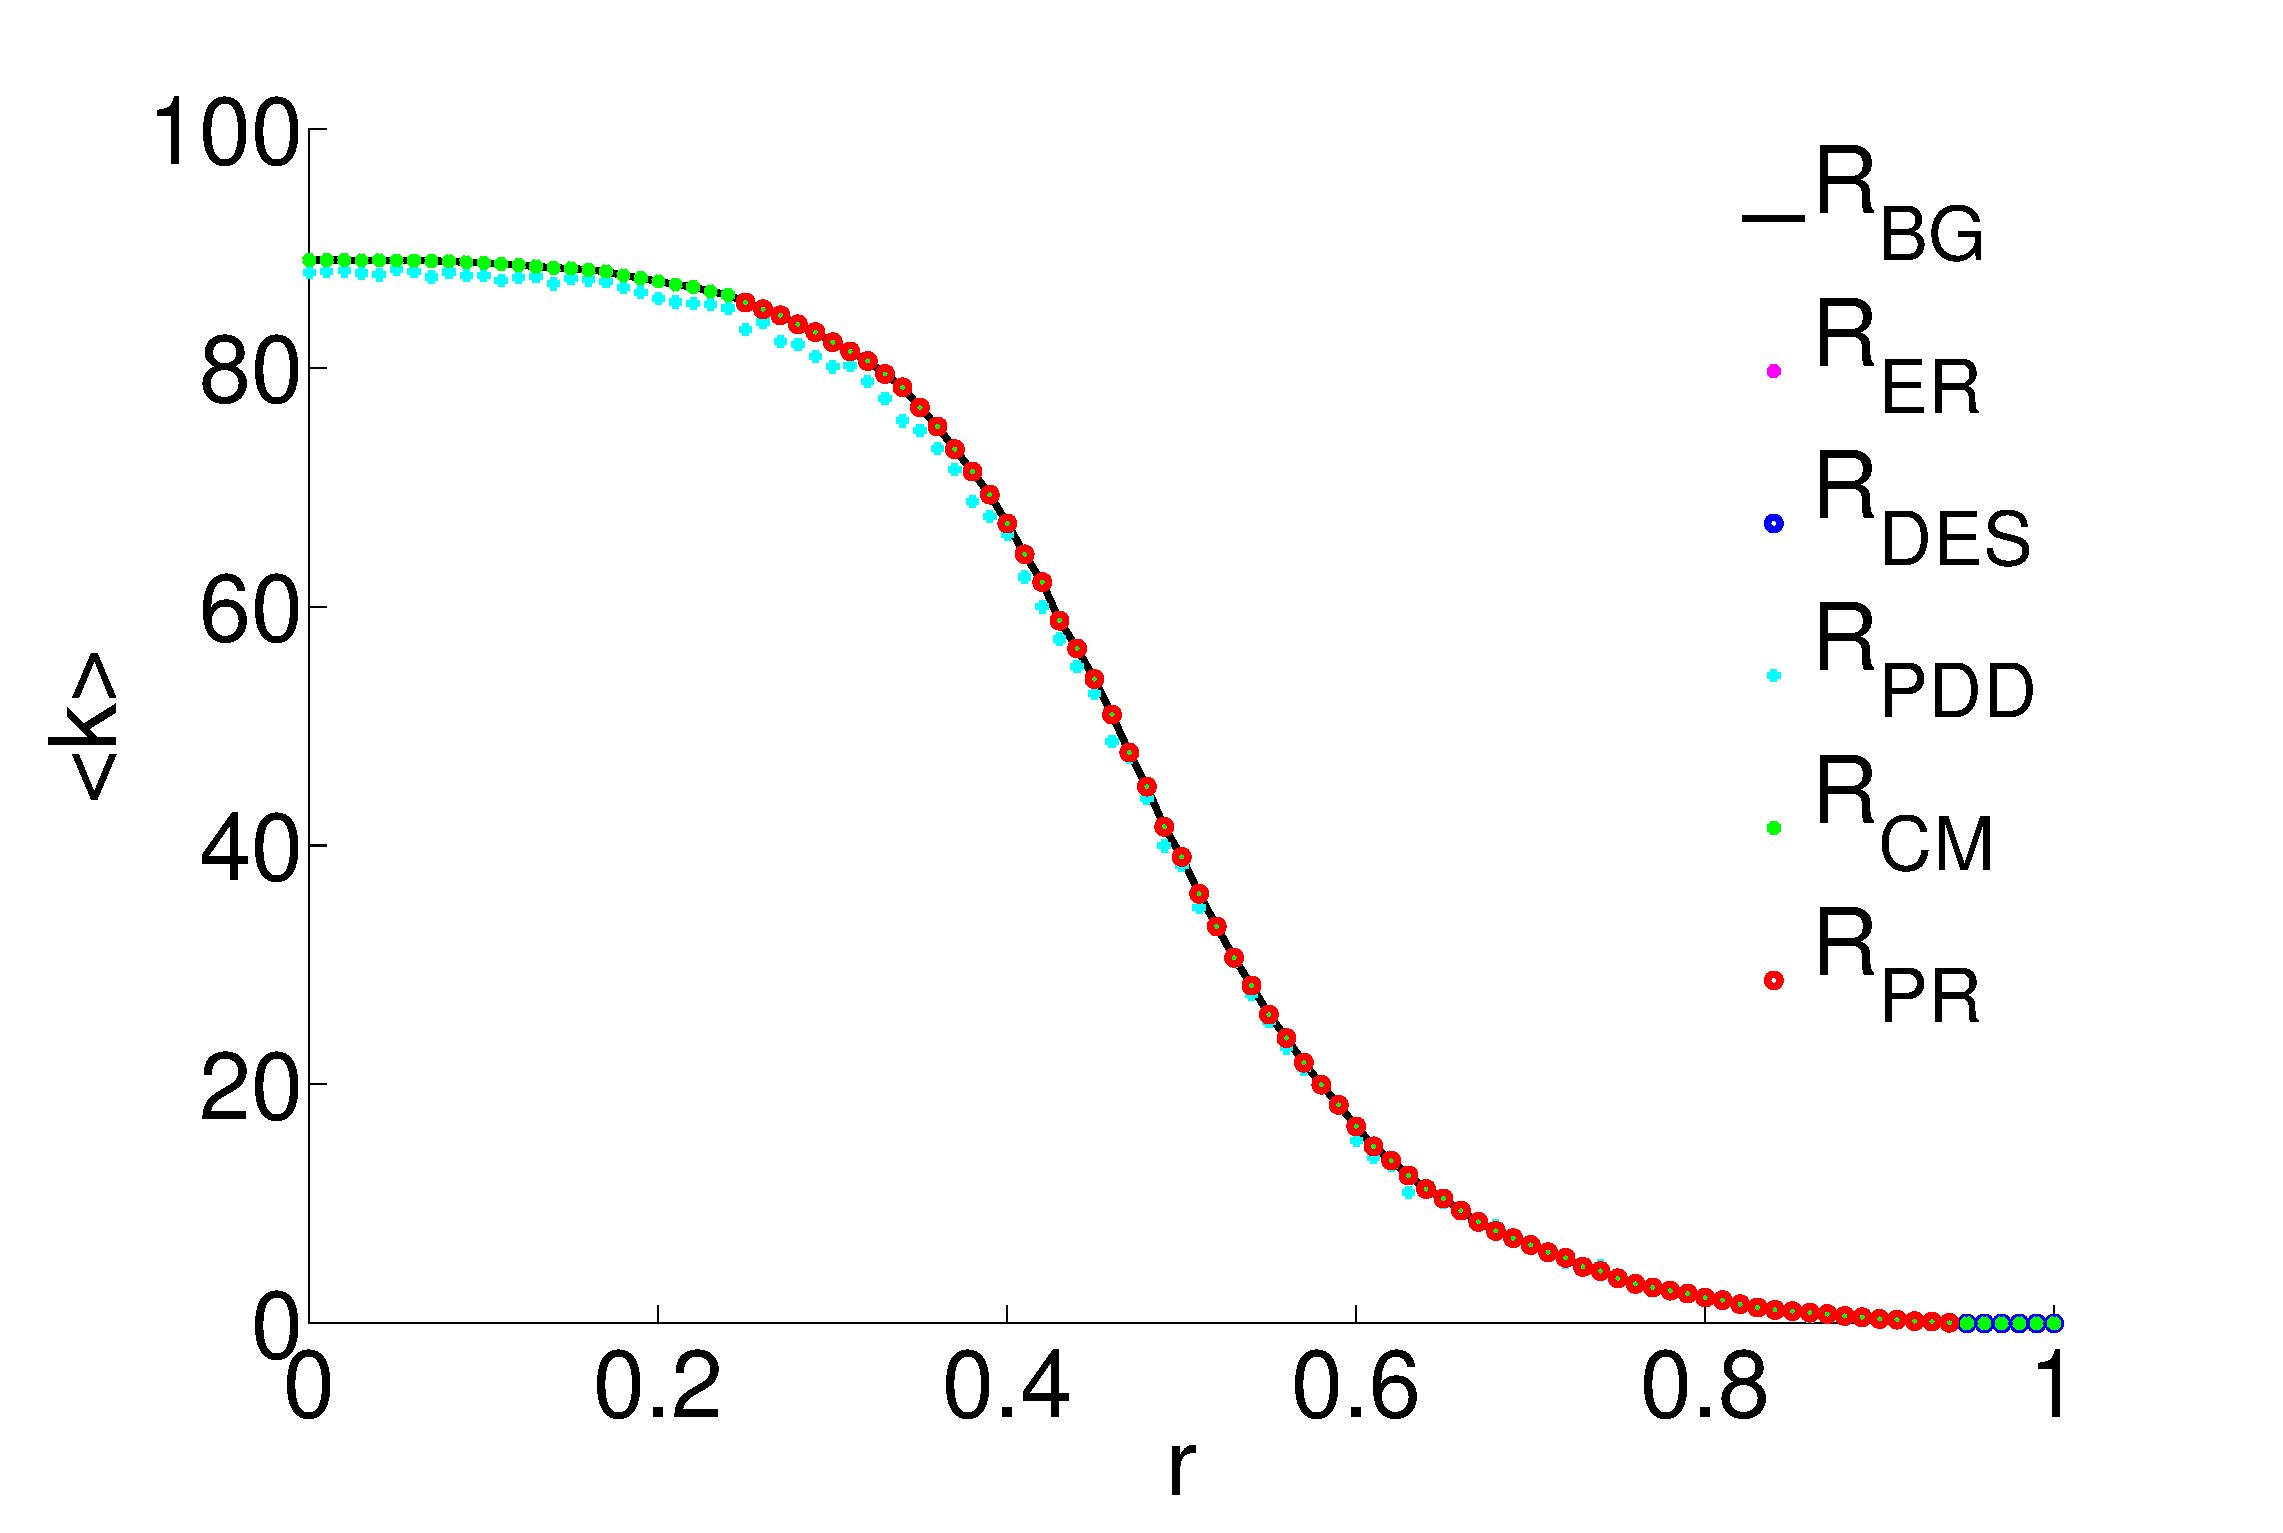
\includegraphics[width=0.45\textwidth, height=60mm]{Figures\Degree_Average_Fnc.eps} 
%
%    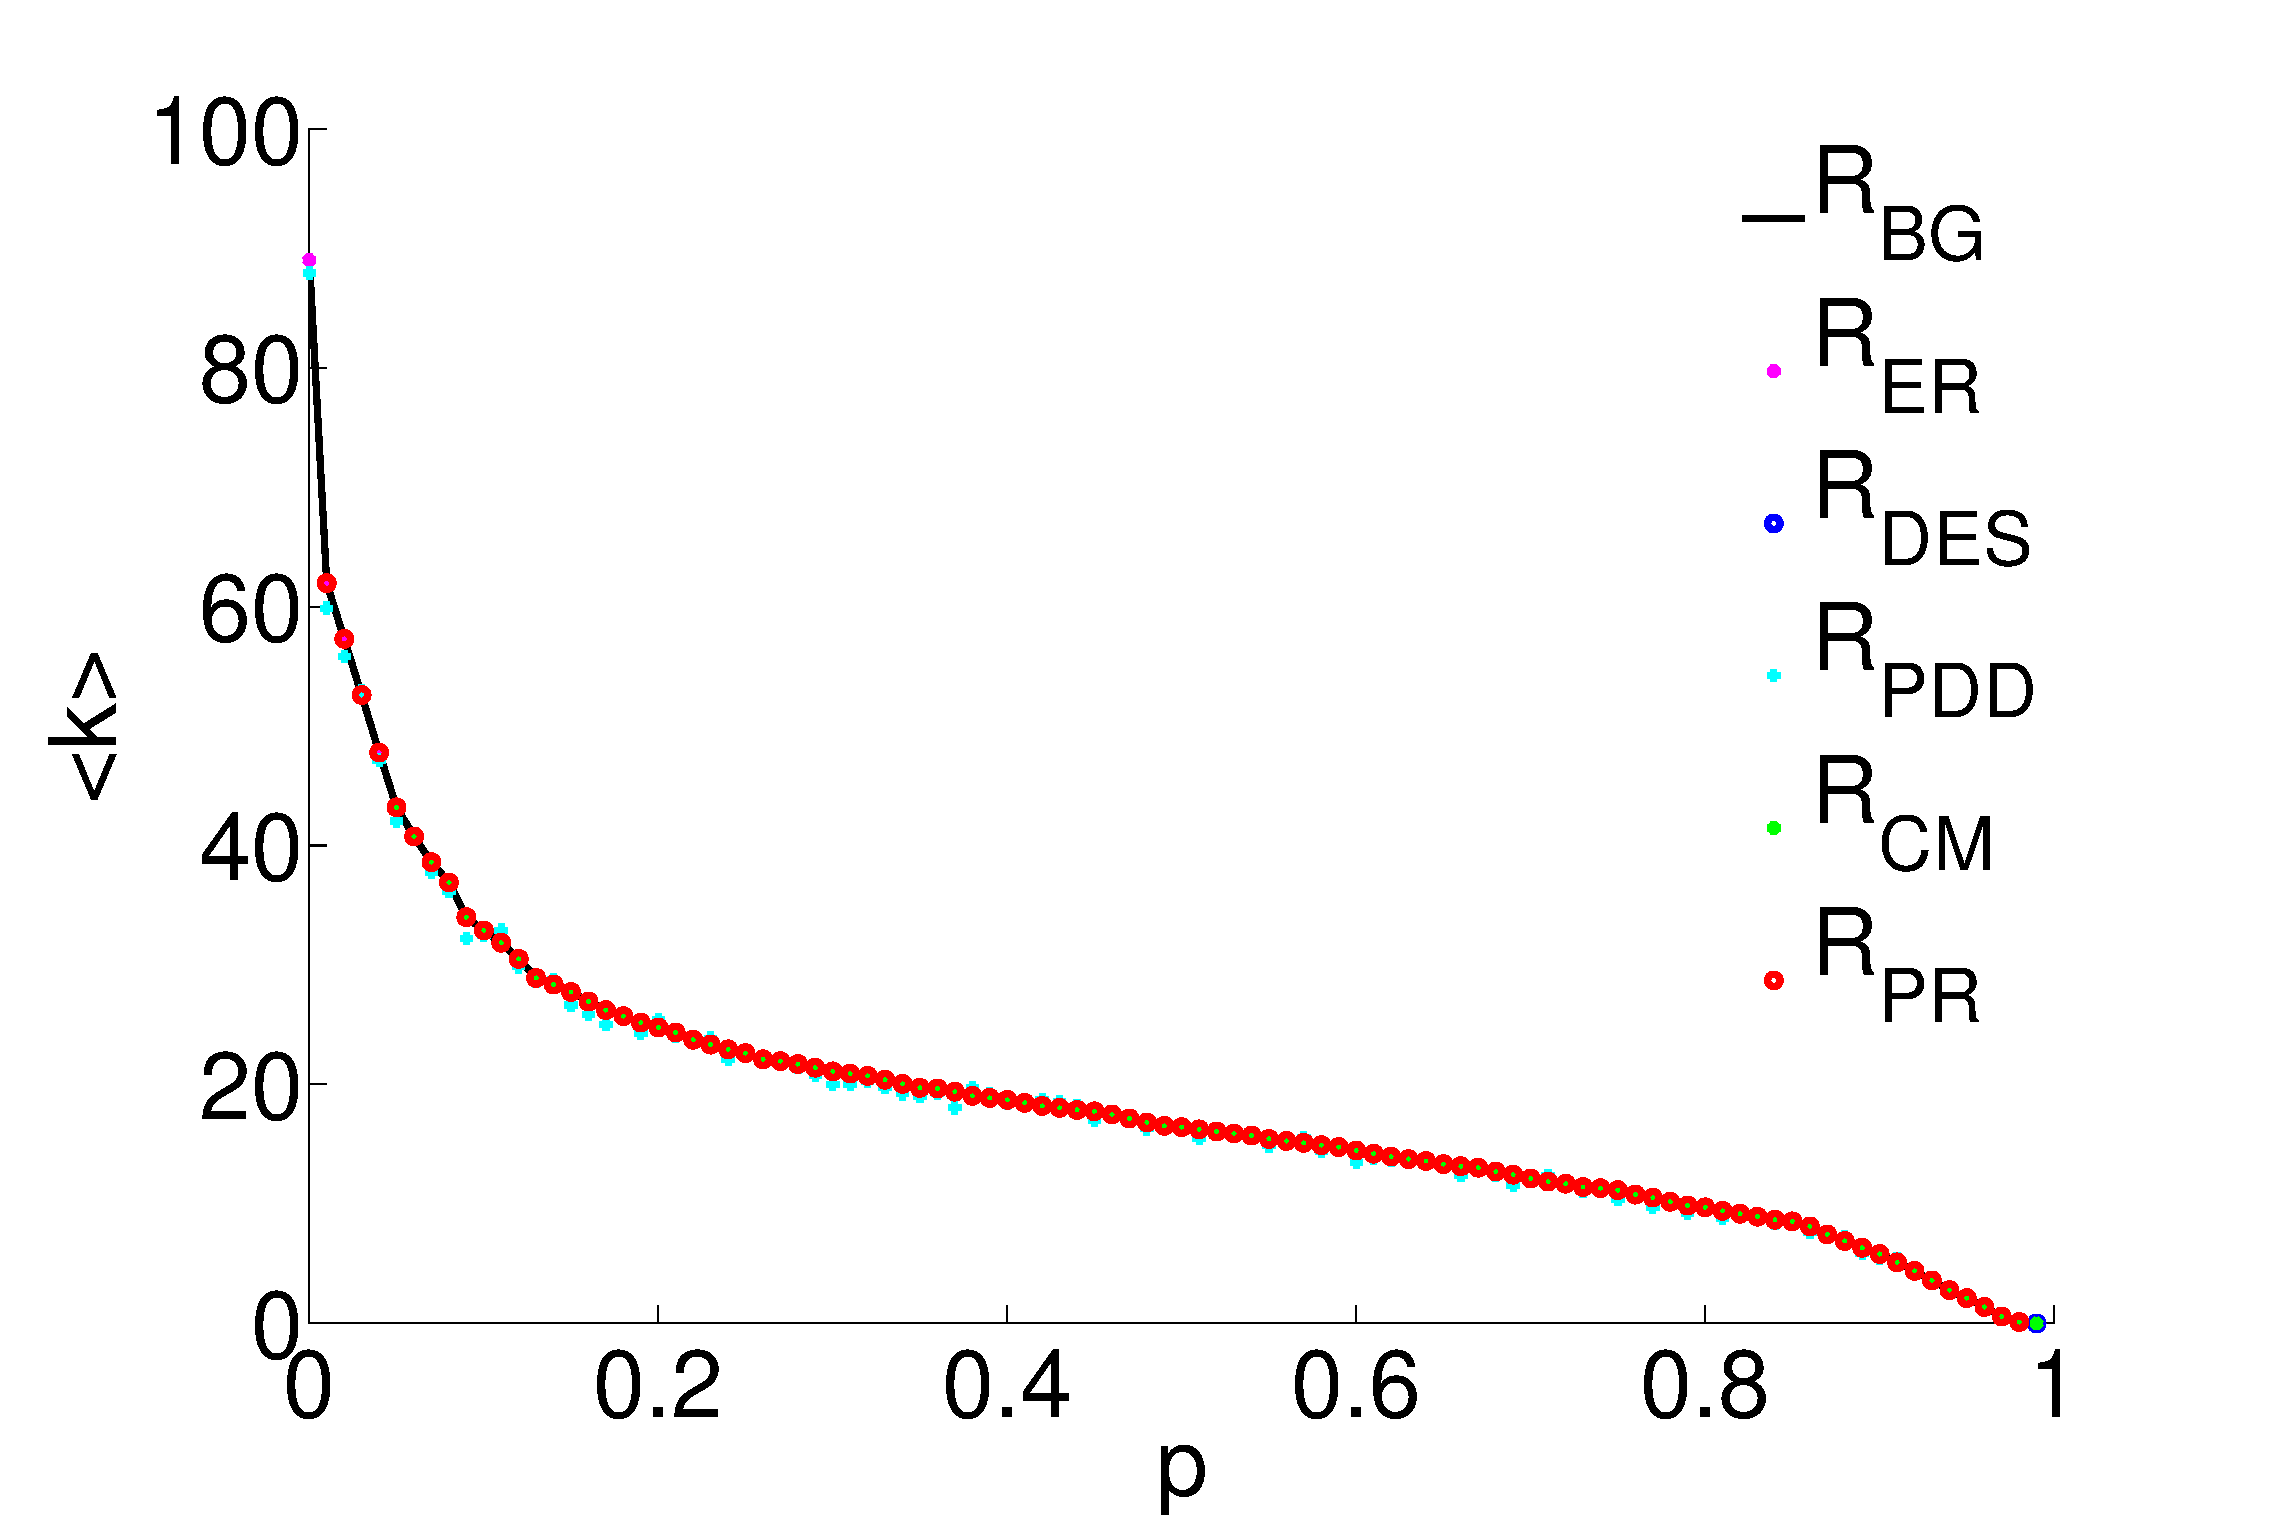
\includegraphics[width=0.45\textwidth, height=60mm]{Figures\Degree_Average_Stru.eps}
%
% 
% \label{figur}\caption{Average degrees of the original network and the randomized networks. Left: $R0$ corresponds to the graph of FCM (source is $A\_aal.txt$), right: $R0$ is that of ACM (source is $acp\_w.txt$). Successful $r$ ranges for randomization methods of FCM :  $r_{Ra}=[0,1]$ , $r_{Rd} = [0.25,1.00]$, $r_{Rg} = [0,1.00]$ , $r_{Rh} = [0,1.00]$ , $r_{Rk} = [0.08,0.94]$. Successful $p$ ranges of ACM : $p_{Ra}=[0,0.99]$, $p_{Rd}=[0.01 , 0.99]$, $p_{Rg}=[0, 0.99]$ , $p_{Rh}=[0.05 , 0.98]$. }
%
%\end{figure}
%%



\begin{figure}[htbp]
 
  \centering
	 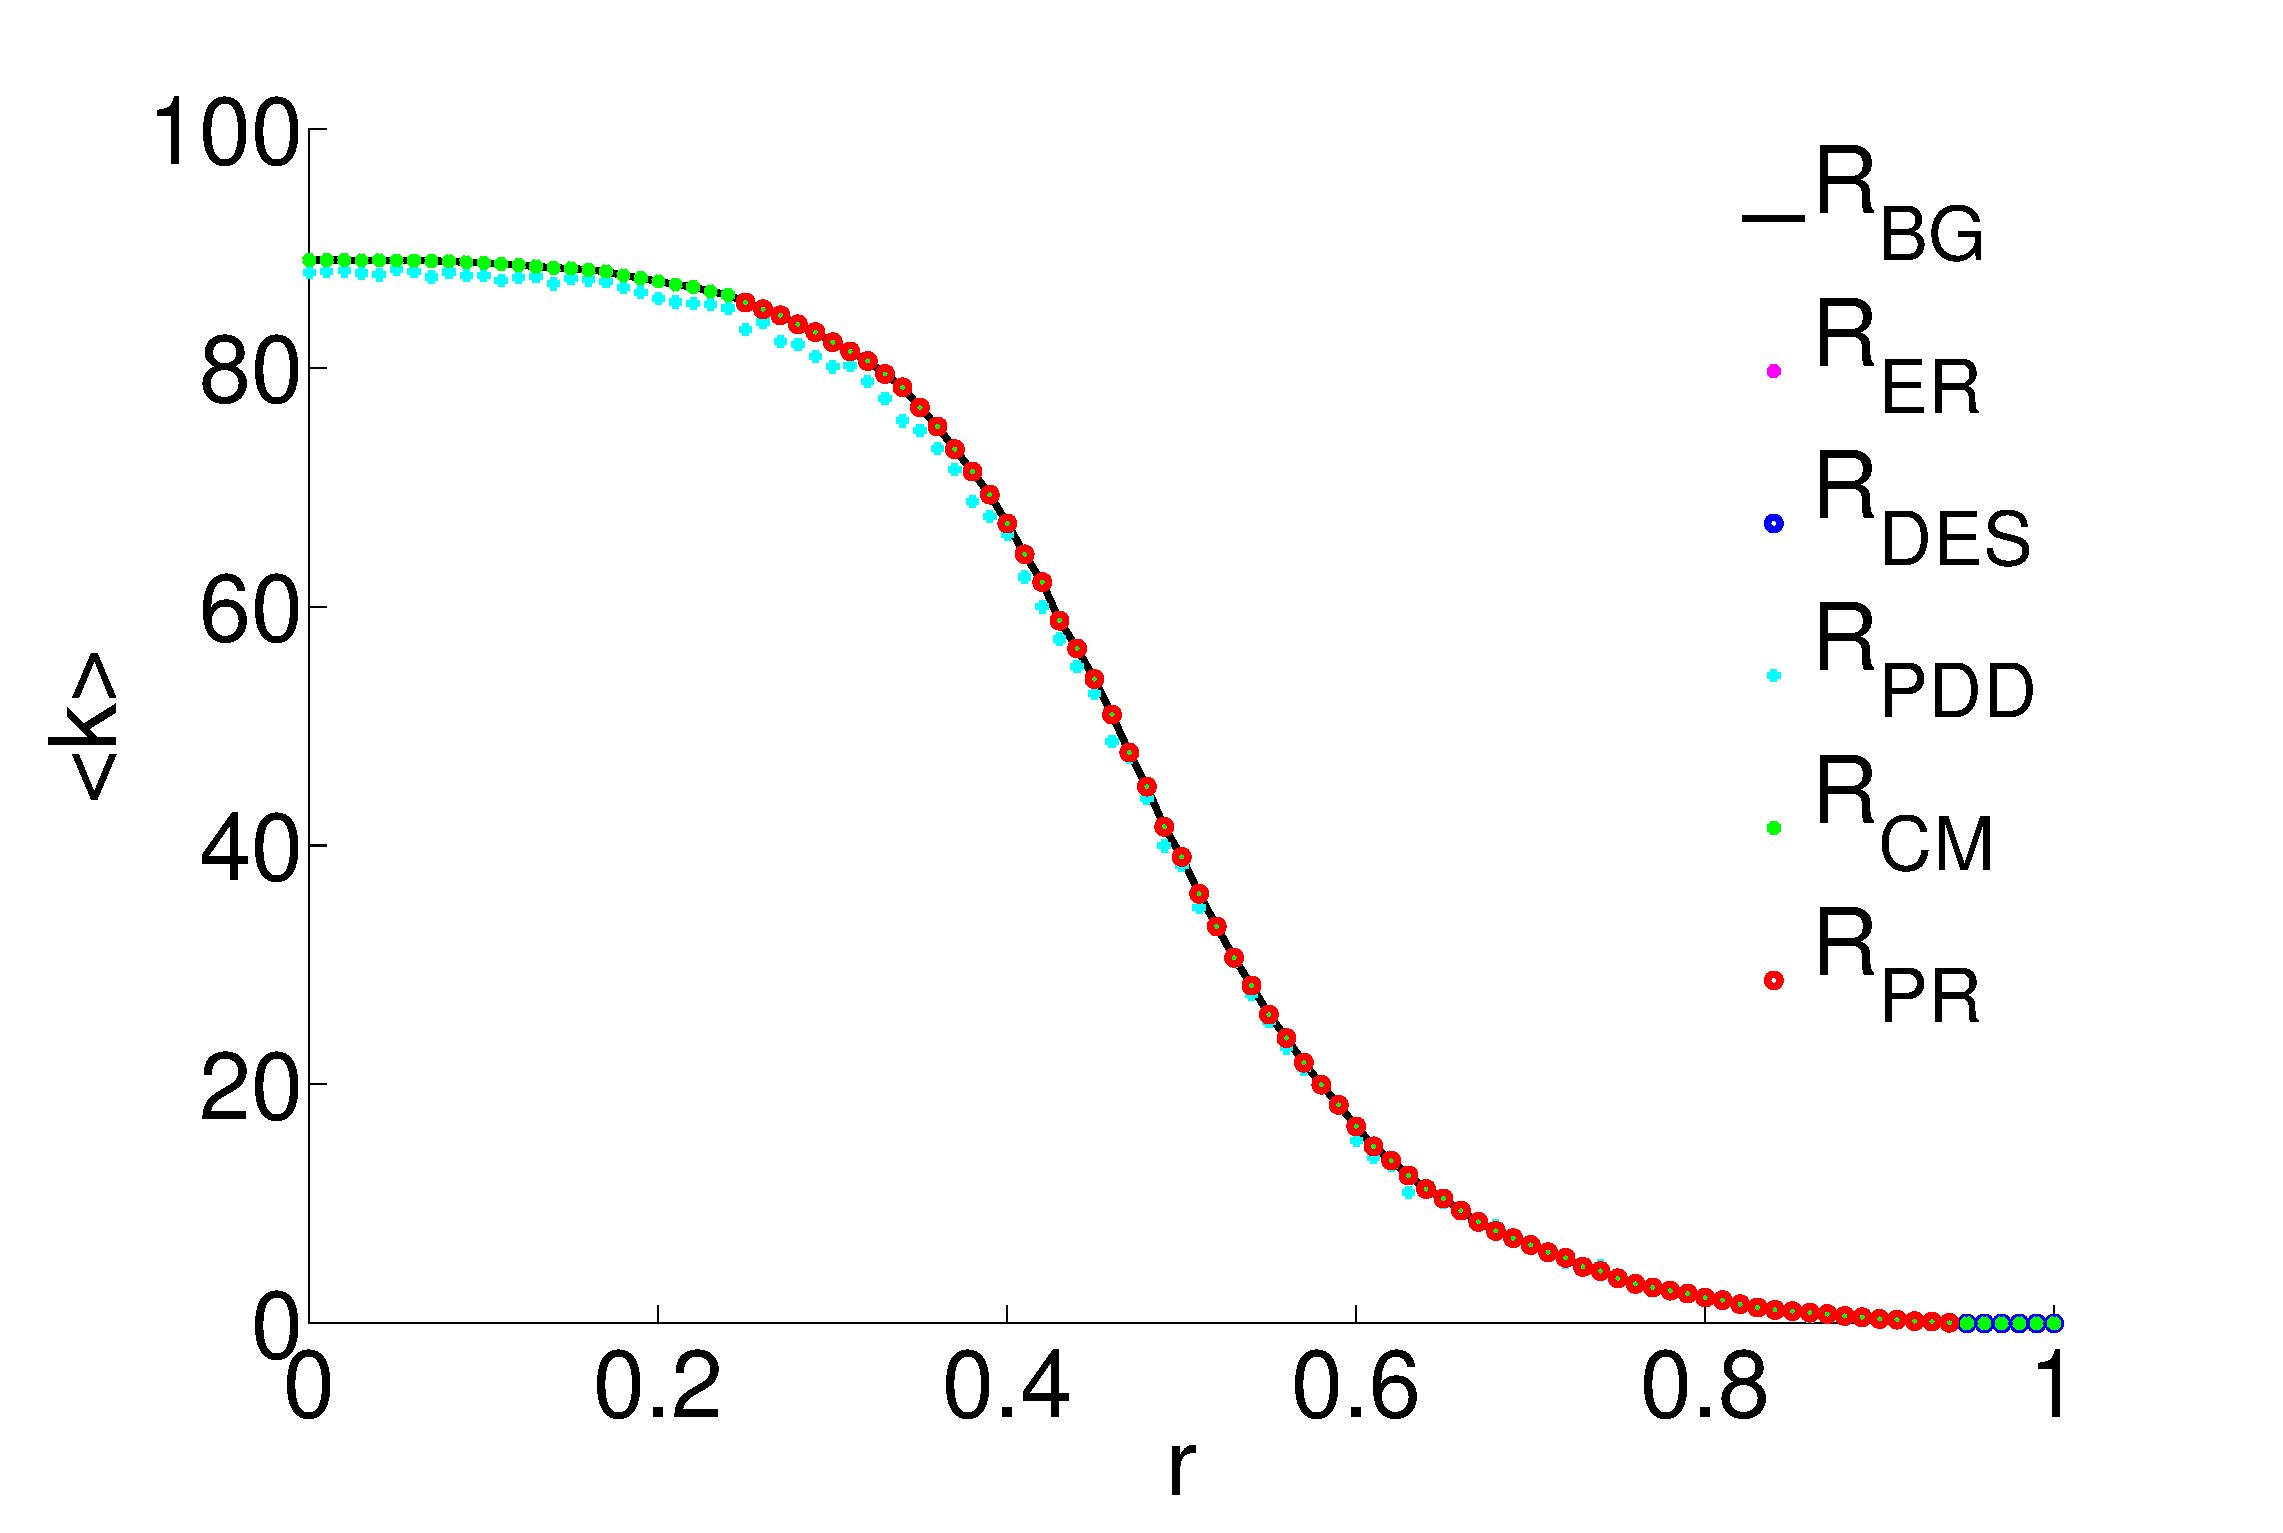
\includegraphics[width=0.49\textwidth]{../reports/MSc_01_report/Degree_Average_Fnc.eps}
	 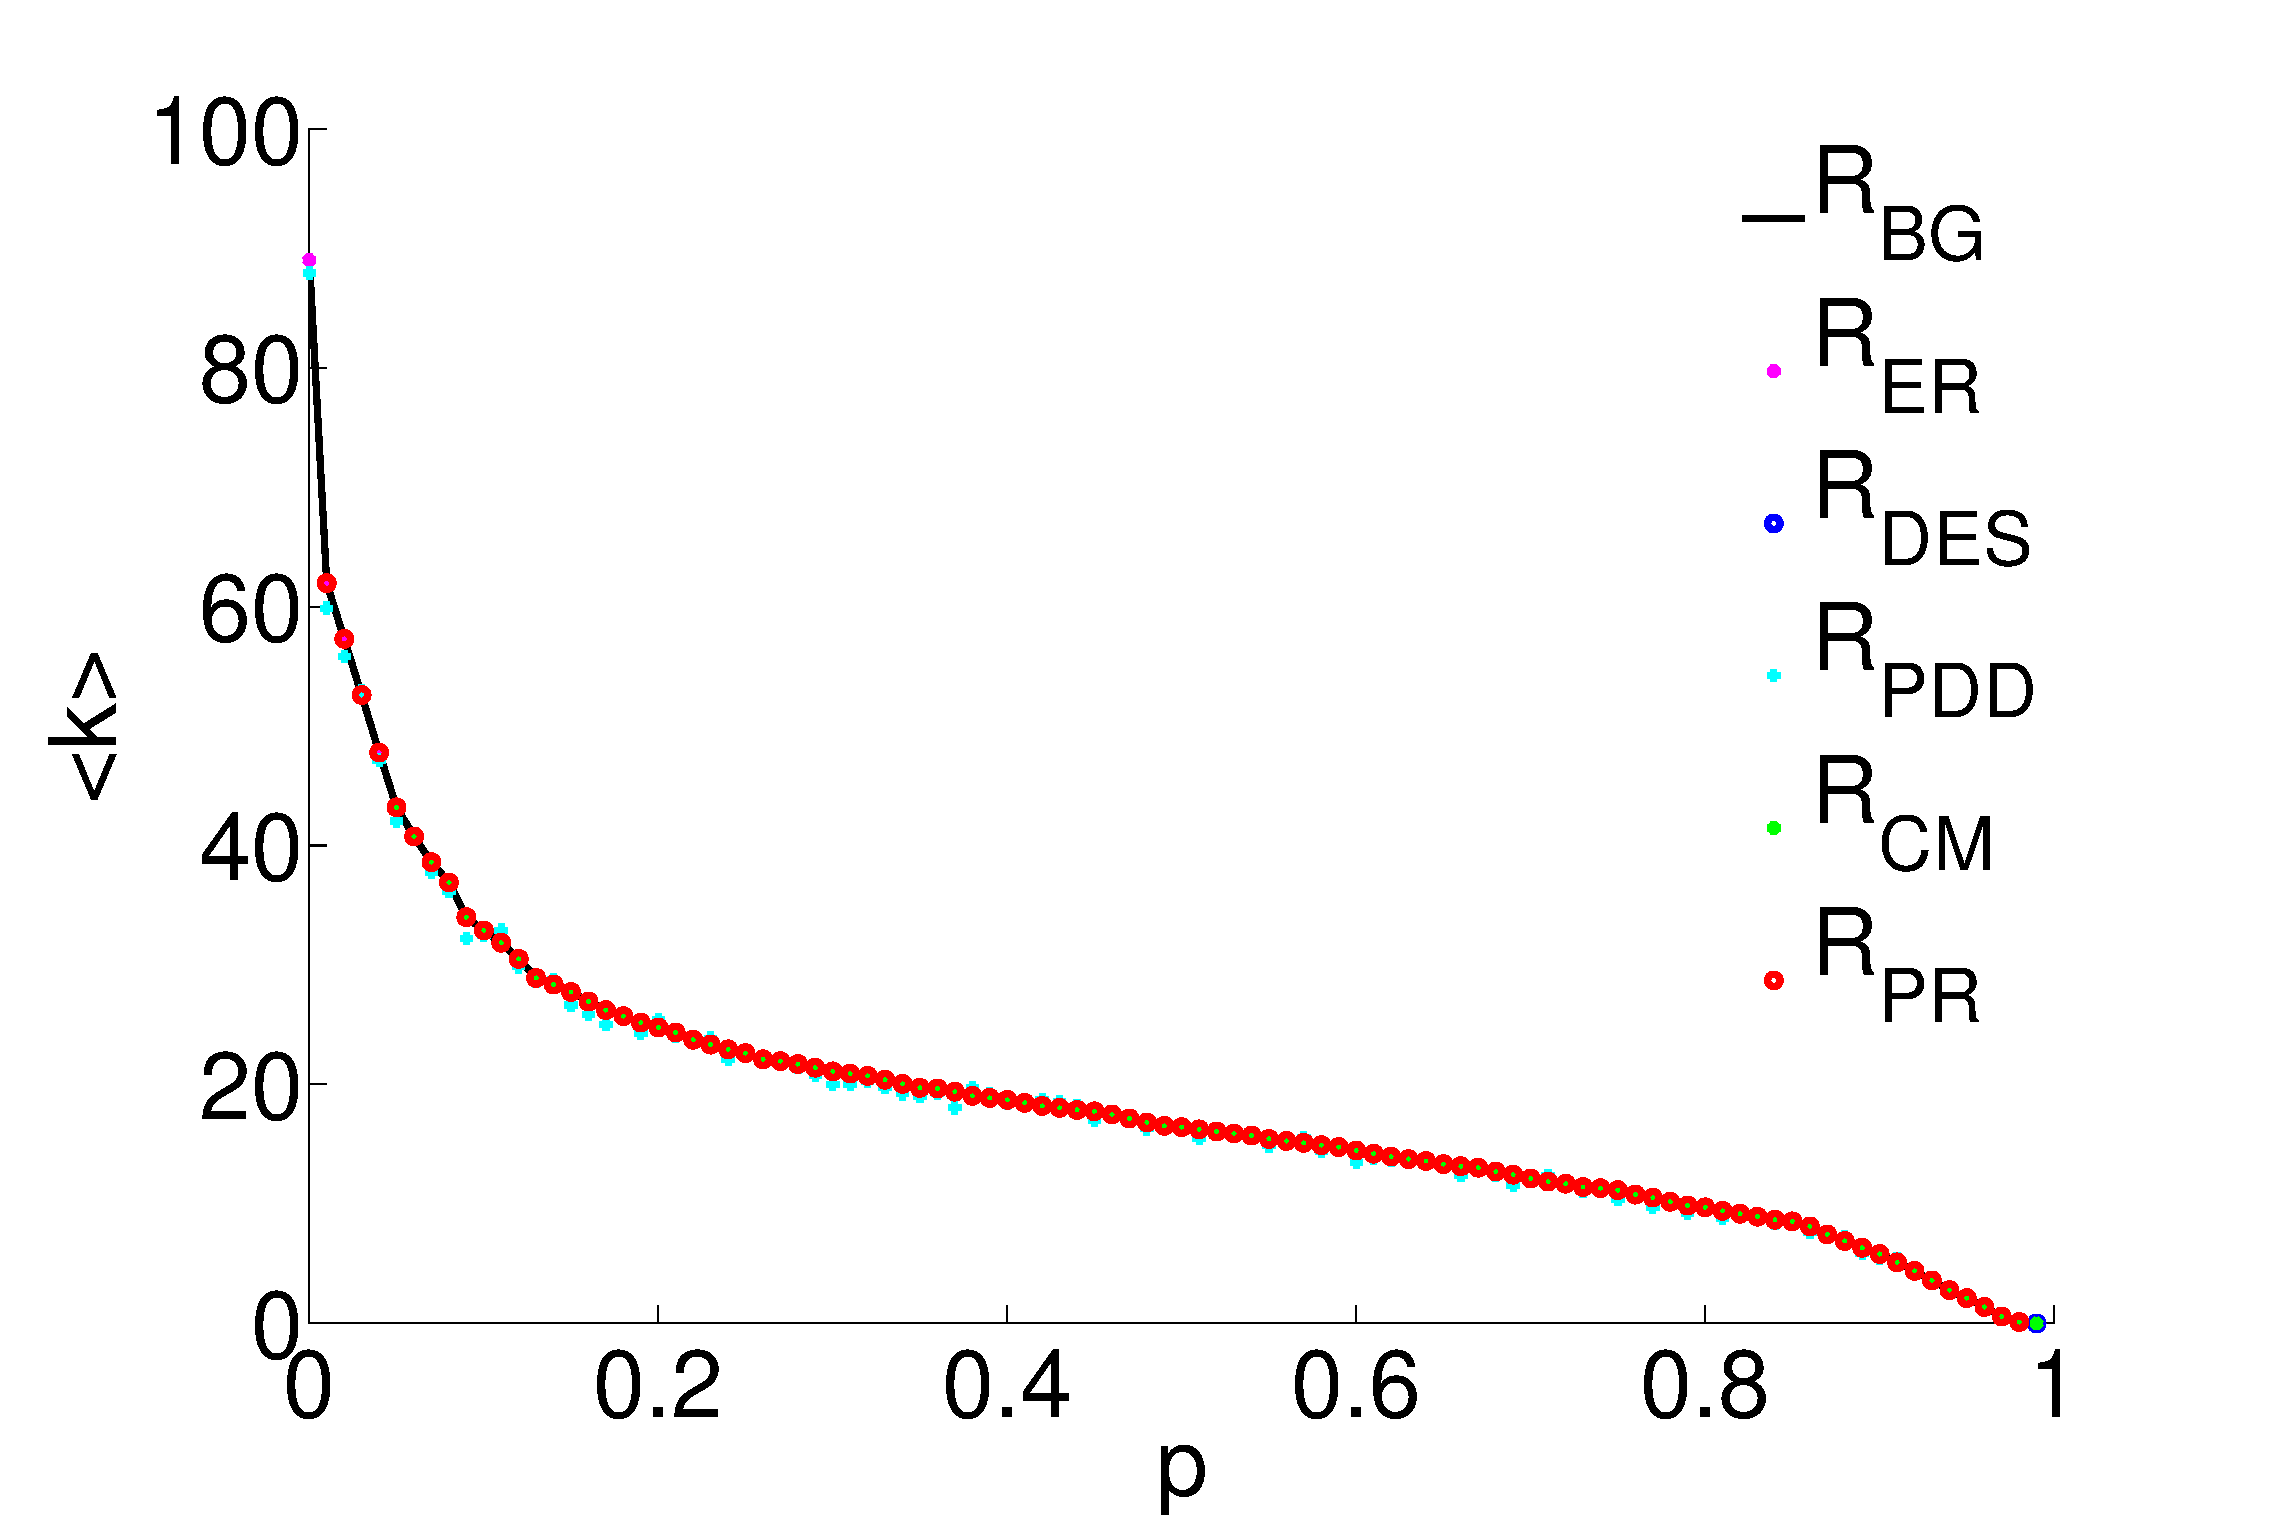
\includegraphics[width=0.49\textwidth]{../reports/MSc_01_report/Degree_Average_Stru.eps}
  \caption[Average Degree]{Average degrees of the brain network and the randomized networks, FCM related graphs on the left, ACM related graphs on the right. Successful $r$ ranges for randomization methods of FCM :  $r_{Ra}=[0,1]$ , $r_{Rd} = [0.25,1.00]$, $r_{Rg} = [0,1.00]$ , $r_{Rh} = [0,1.00]$ , $r_{Rk} = [0.08,0.94]$. Successful $p$ ranges of ACM : $p_{Ra}=[0,0.99]$, $p_{Rd}=[0.01 , 0.99]$, $p_{Rg}=[0, 0.99]$ , $p_{Rh}=[0.05 , 0.98]$.} 
    \label{fig:Average Degree}
 	
\end{figure}  


Degree is one of the statistical tools to measure the centrality of network. The higher the average degree is, the more interaction the nodes in the graph have. 

Increasing threshold and probability values diminishes number of edges inverse sigmoidally. As long as the total node numbers, total edge numbers and networks density are all preserved while constructing the random graphs, the average degree remains the same. 

\section{Shortest Pathway}
Shortest pathway $d_{ij}$ is a measure of integration in the network, opposite to the segregation measures. It corresponds to the shortest path length between two nodes in an unweighted graph,  

\begin{equation}
d_{ij} = \sum\limits_{a_{uv} \epsilon g_{i\leftrightarrow j} } a_{uv}
\end{equation}
where $g_{i\leftrightarrow j}$ is the shortest path between nodes $i$ and $j$, $d_{ij}$ is assumed to be $\infty$ for disconnected pairs \citep{RUB10}.


\begin{figure}[htbp]
 
  \centering
	 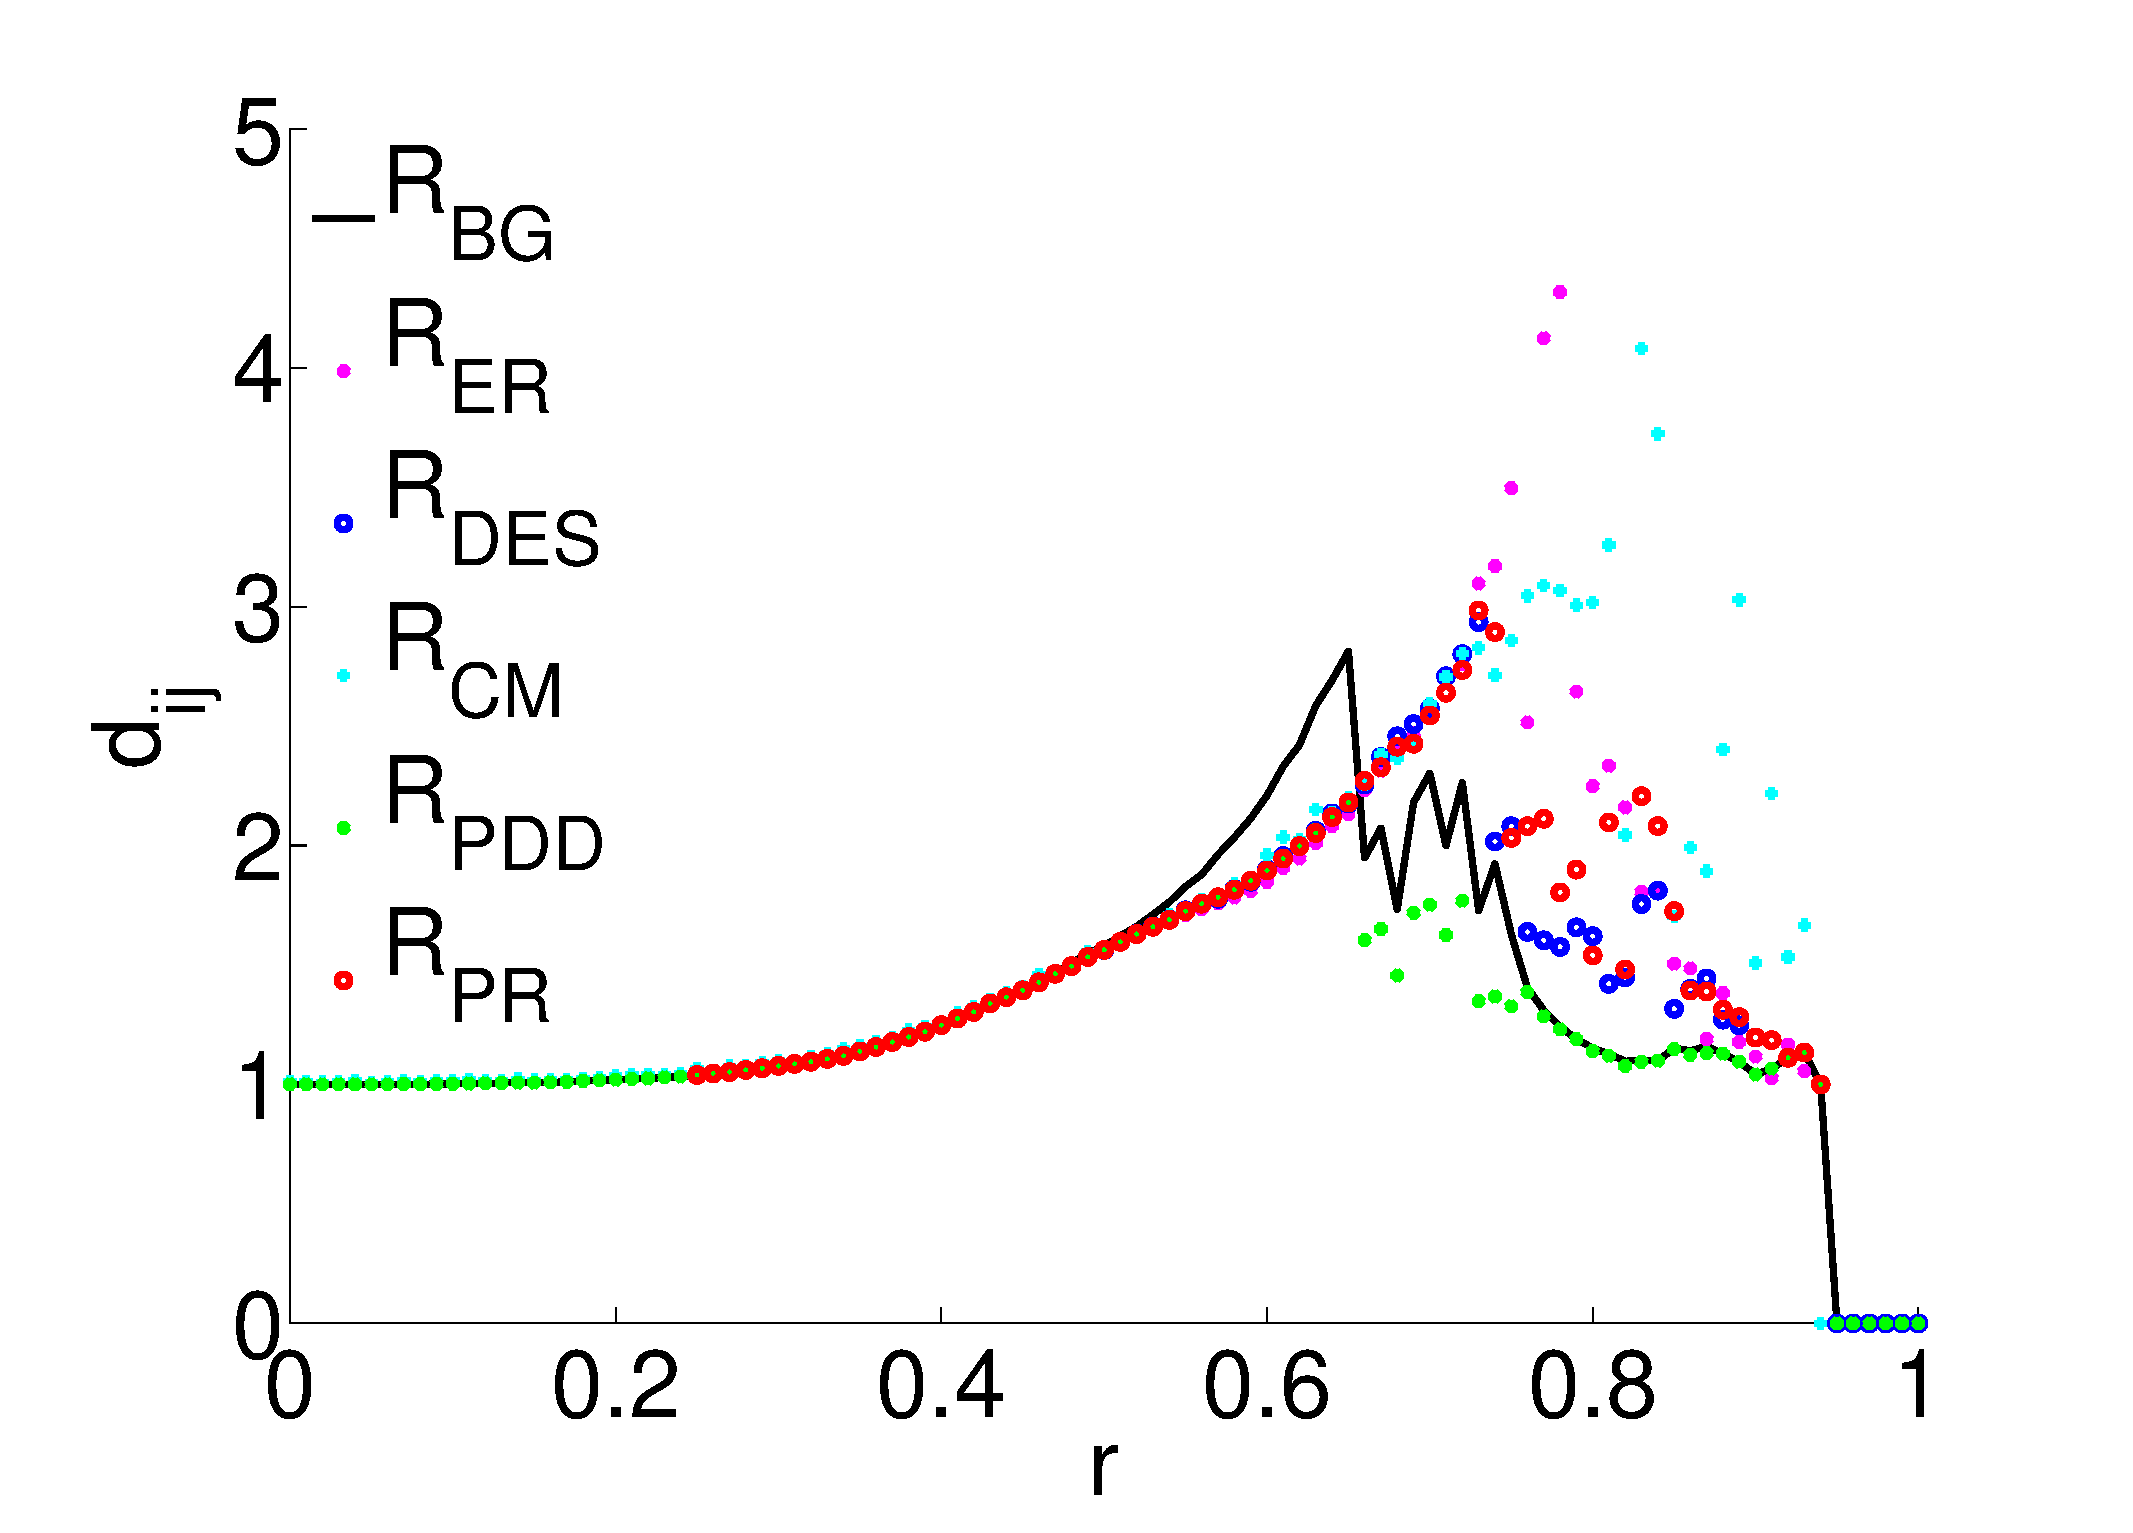
\includegraphics[width=0.49\textwidth]{../reports/MSc_01_report/Shortest_Pathway_Fnc.eps}
	 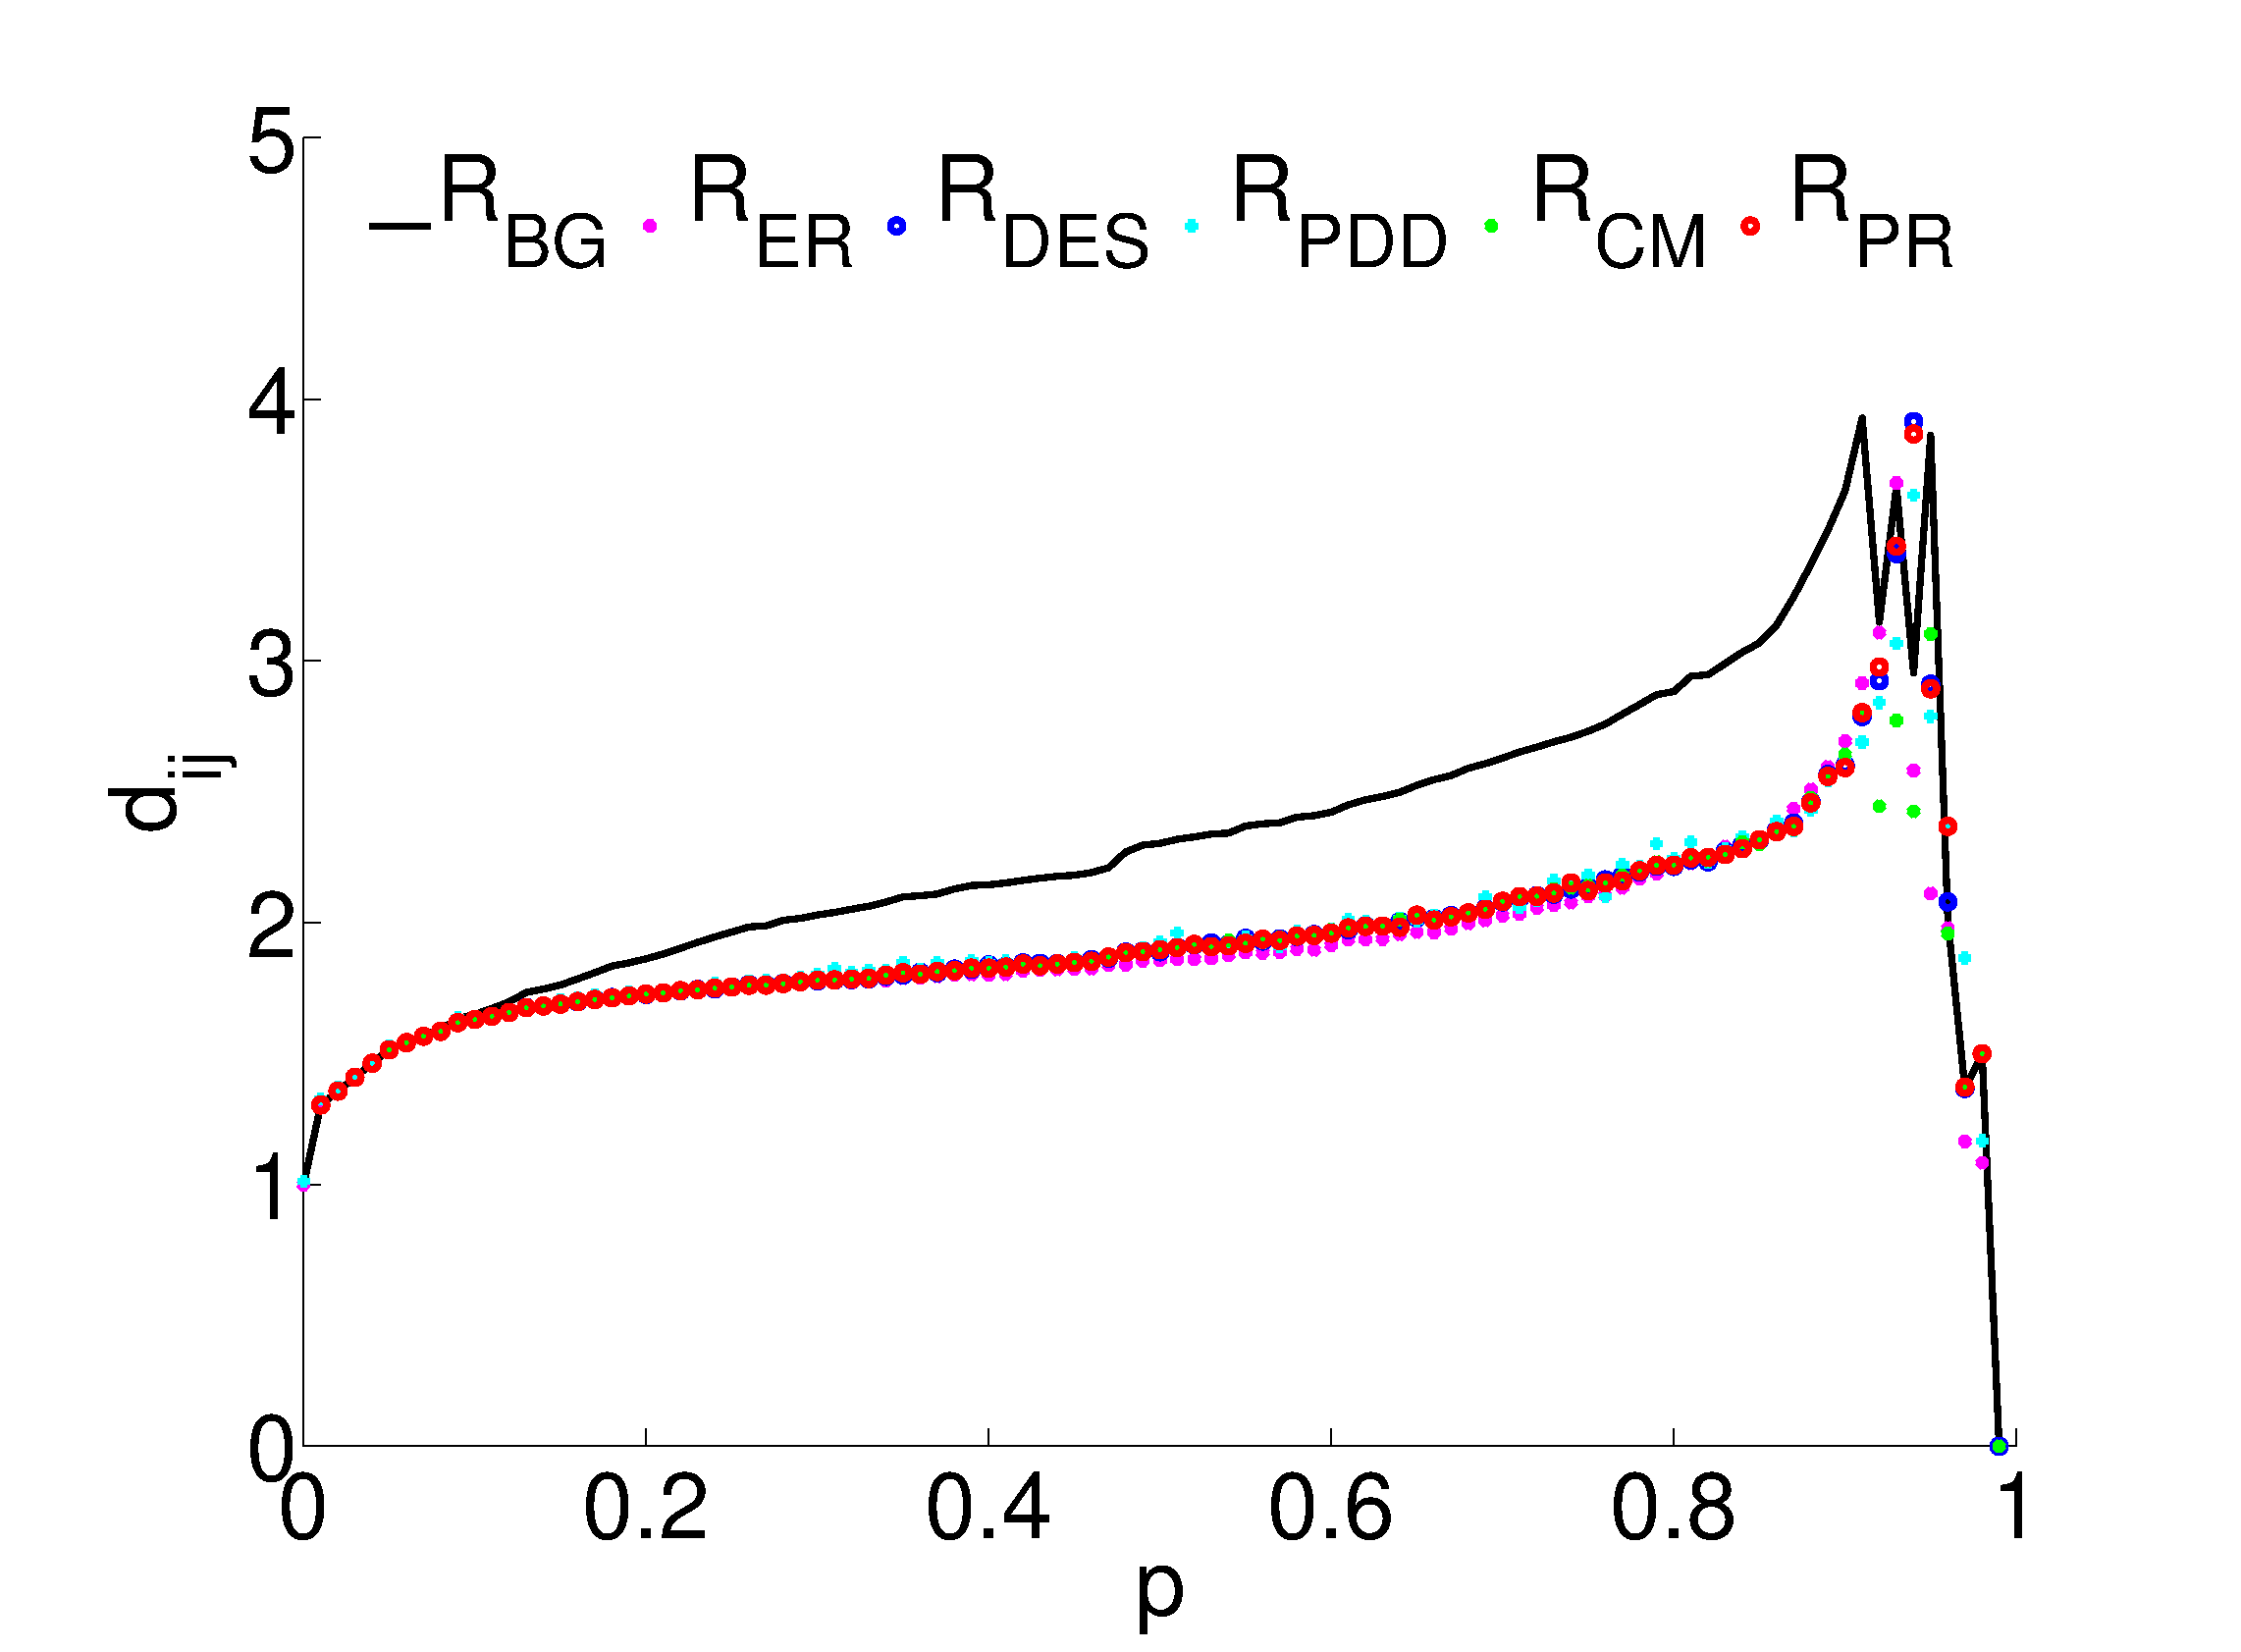
\includegraphics[width=0.49\textwidth]{../reports/MSc_01_report/Shortest_Pathway_Stru.eps}
  \caption[Shortest Pathway]{Shortest pathway of the brain graphs and random graphs, FCM graphs on the left and ACM graphs on the right.} 
    \label{fig:Shortest Pathway}
 	
\end{figure}  


The $R0$ network of FCM seems to be less segregated than the randomized networks while $r$ lies between $[0.65,0.95]$. This is the threshold value at which the $R0$ network of FCM begins to get multiple components. The $R0$ network of ACM tends to be more segregated than its random networks. Whenever all the nodes get sparse (approximately $r>0.95$, $p>95$) in both FCM and ACM networks, the shortest pathway is represented as 0. 




\section{Global Efficiency}
The global efficiency $E$ is measured as the average of the inverse shortest pathway,

\begin{equation}
E = \frac{1}{n}\sum\limits_{i \epsilon N} E_i = \frac{1}{n}\sum\limits_{i \epsilon N} \frac{\sum\limits_{j \epsilon N, j\neq i}d_{ij}^{-1}}{n-1 }
\end{equation}

where $E_i$ is the global efficiency of node, $d_{ij}$ is the shortest pathway between nodes $i$ and $j$ \citep{LAT01}. As seen from the equation, global efficiency becomes larger with smaller shortest pathways between nodes. The global efficiency is a measure of the integration in the network. It reveals the strength of connections in a network. Global efficiency measures the ability of a network to transmit information at the global level \citep{XYZDA}.


\begin{figure}[htbp]
 
  \centering
	 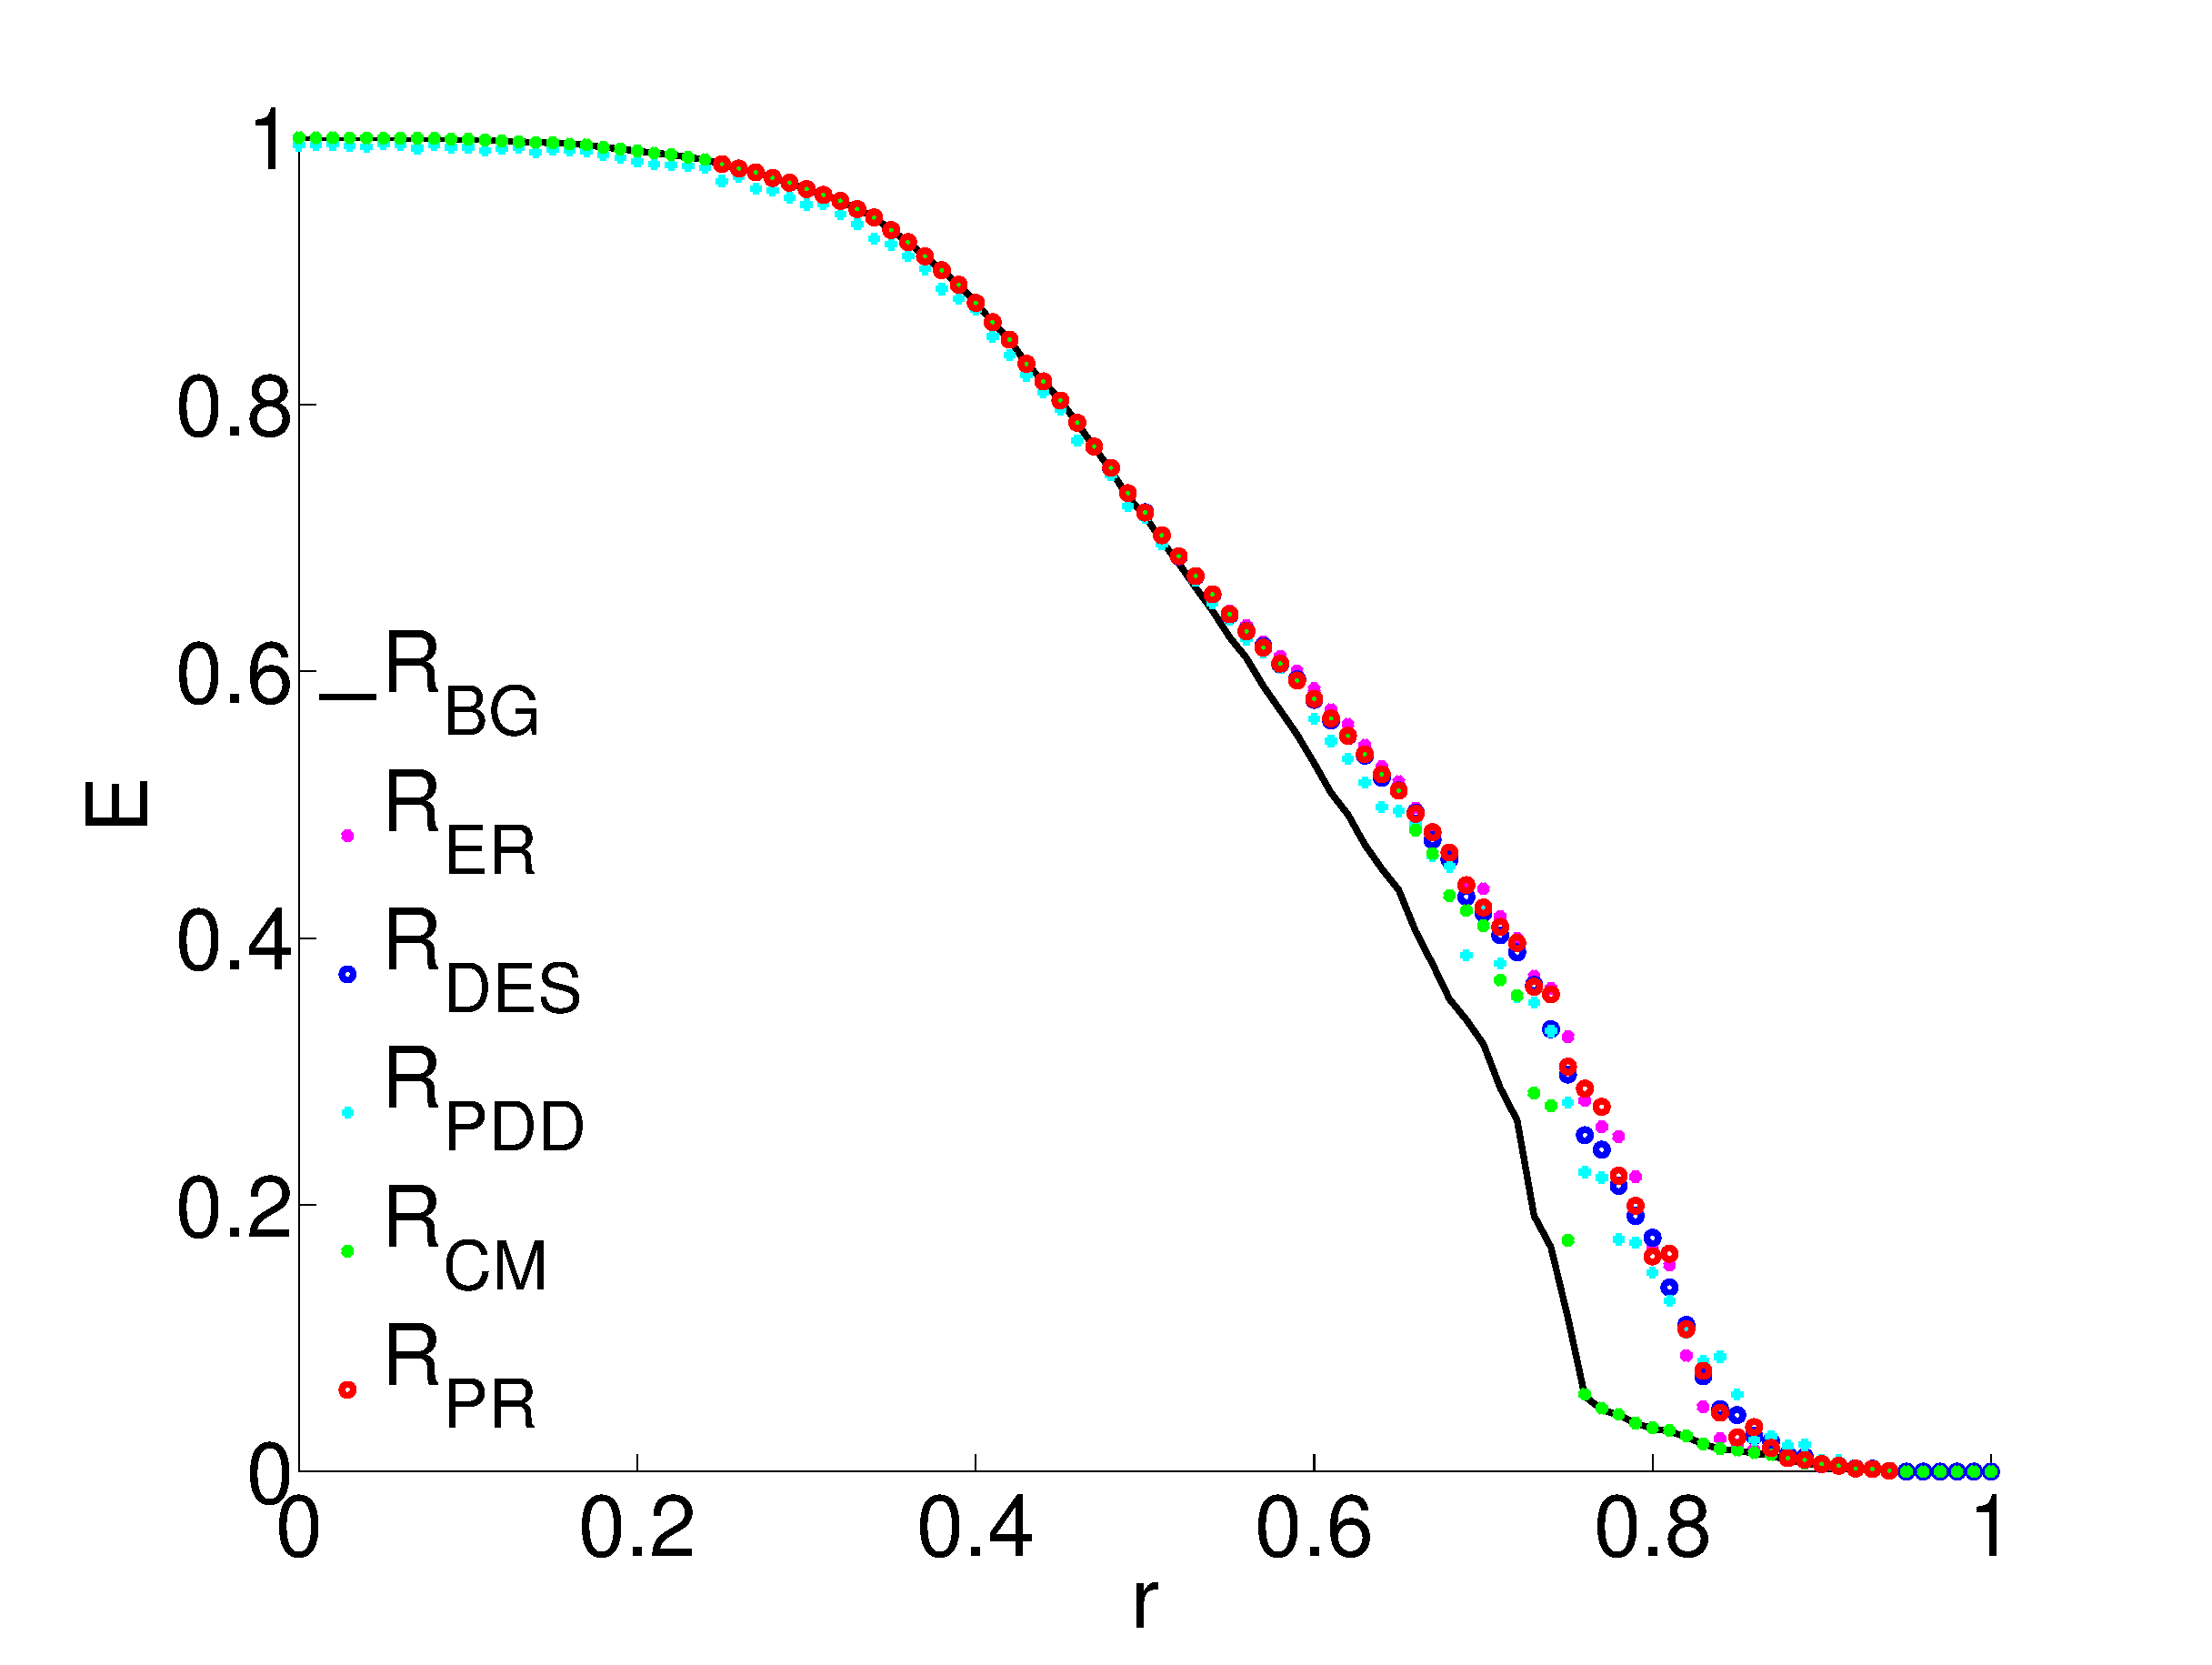
\includegraphics[width=0.49\textwidth]{../reports/MSc_01_report/Global_Efficiency_Average_Fnc.eps}
	 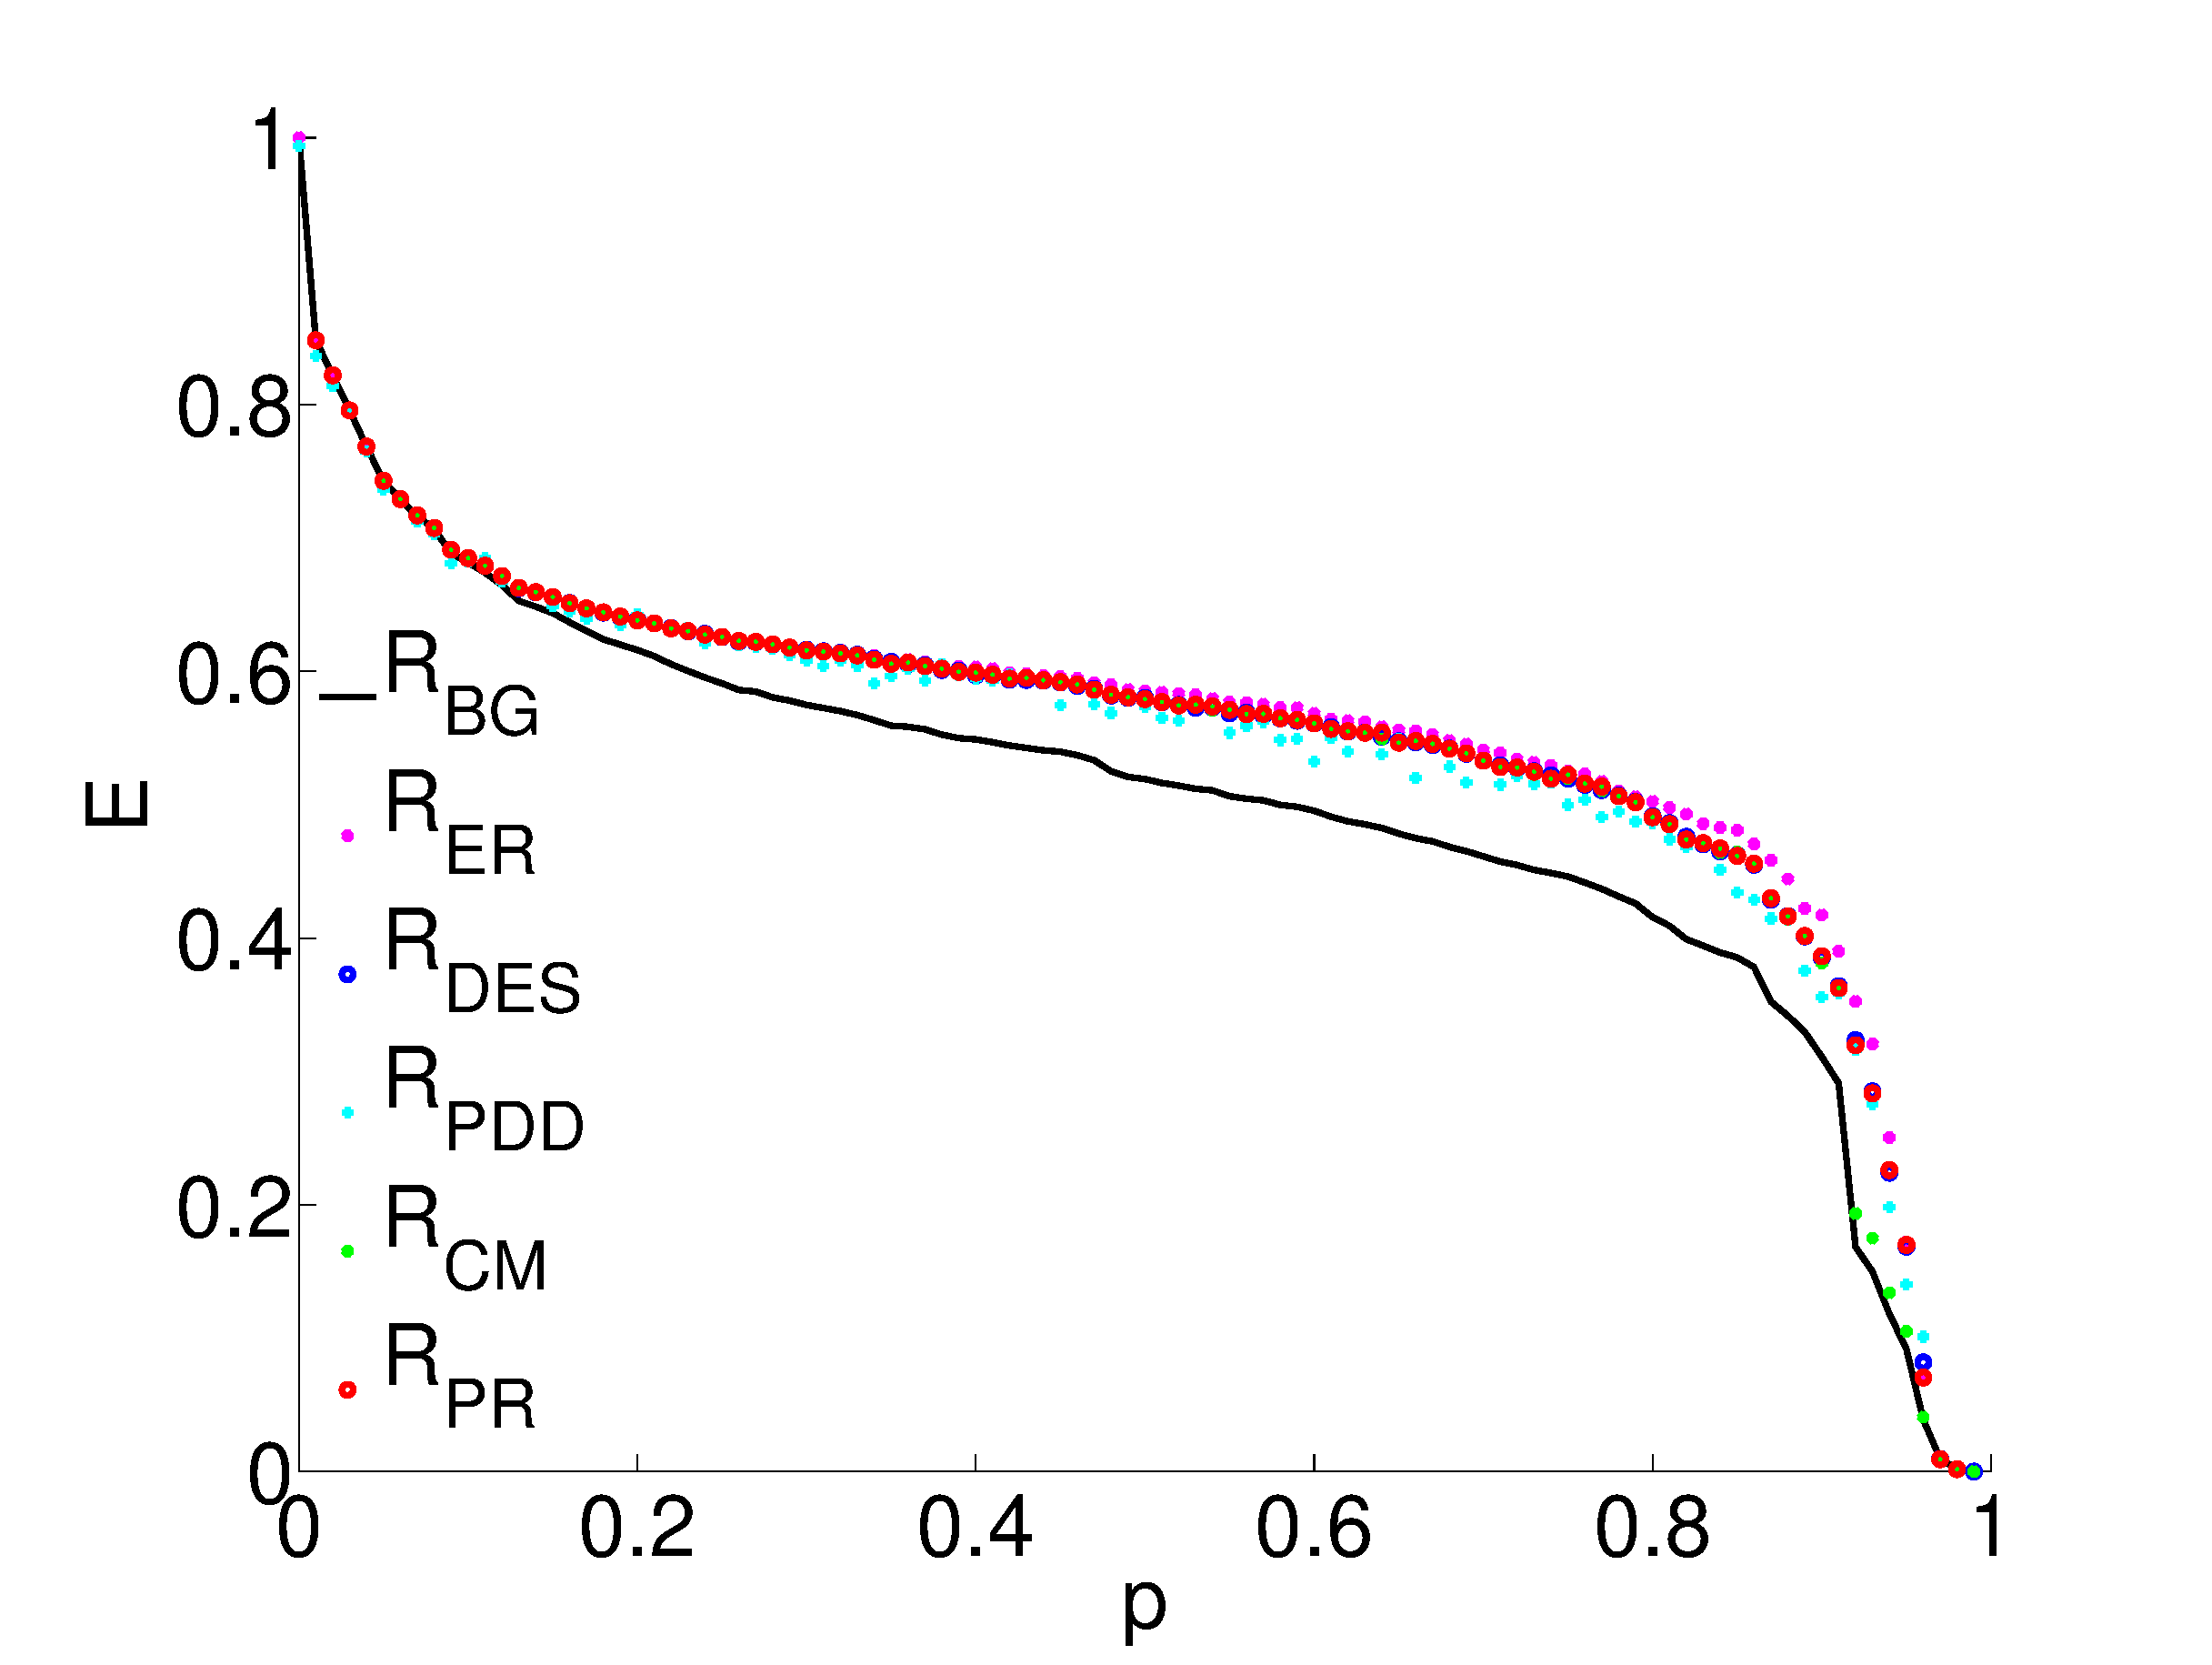
\includegraphics[width=0.49\textwidth]{../reports/MSc_01_report/Global_Efficiency_Average_Stru.eps}
  \caption[Global Efficiency]{Global efficiencies of the original networks and random graphs; FCM on left side, ACM on right side.} 
    \label{fig:Global Efficiency}
 	
\end{figure}

All randomly constructed graphs tend to have in slightly higher $E$ than that of brain graphs. If it is easier to visit a node starting from any other node in the graph, the information transmission capacity is expected to be more robust. When Figure B.2 and B.3 are compared, it can be inferred that higher $d_{ij}$ values reveals lower global efficiency in a network. 



\section{Local Efficiency}
The local efficiency $E_{loc}$ is measured as the average of inverse shortest pathways between nodes in neighborhood of a specific node, 

\begin{equation}
E_{loc} = \frac{1}{n}\sum\limits_{i \epsilon N} E_{loc,i} = \frac{1}{n}\sum\limits_{i \epsilon N} \frac{\sum\limits_{j,h \epsilon N, j\neq i} a_{ij} a_{ih}[d_{jh}(N_i)]^{-1}}{k_i(k_i - 1) }
\end{equation}

where $E_{loc,i}$ is the local efficiency of node $i$, $d_{jh}(N_i)$ is the shortest pathway between nodes $j$ and $h$, which are located in neighborhood of node $i$ \citep{LAT01}. Local efficiency measures the ability of a network to transmit information at the local level \citep{XYZDA}.


\begin{figure}[htbp]
 
  \centering
	 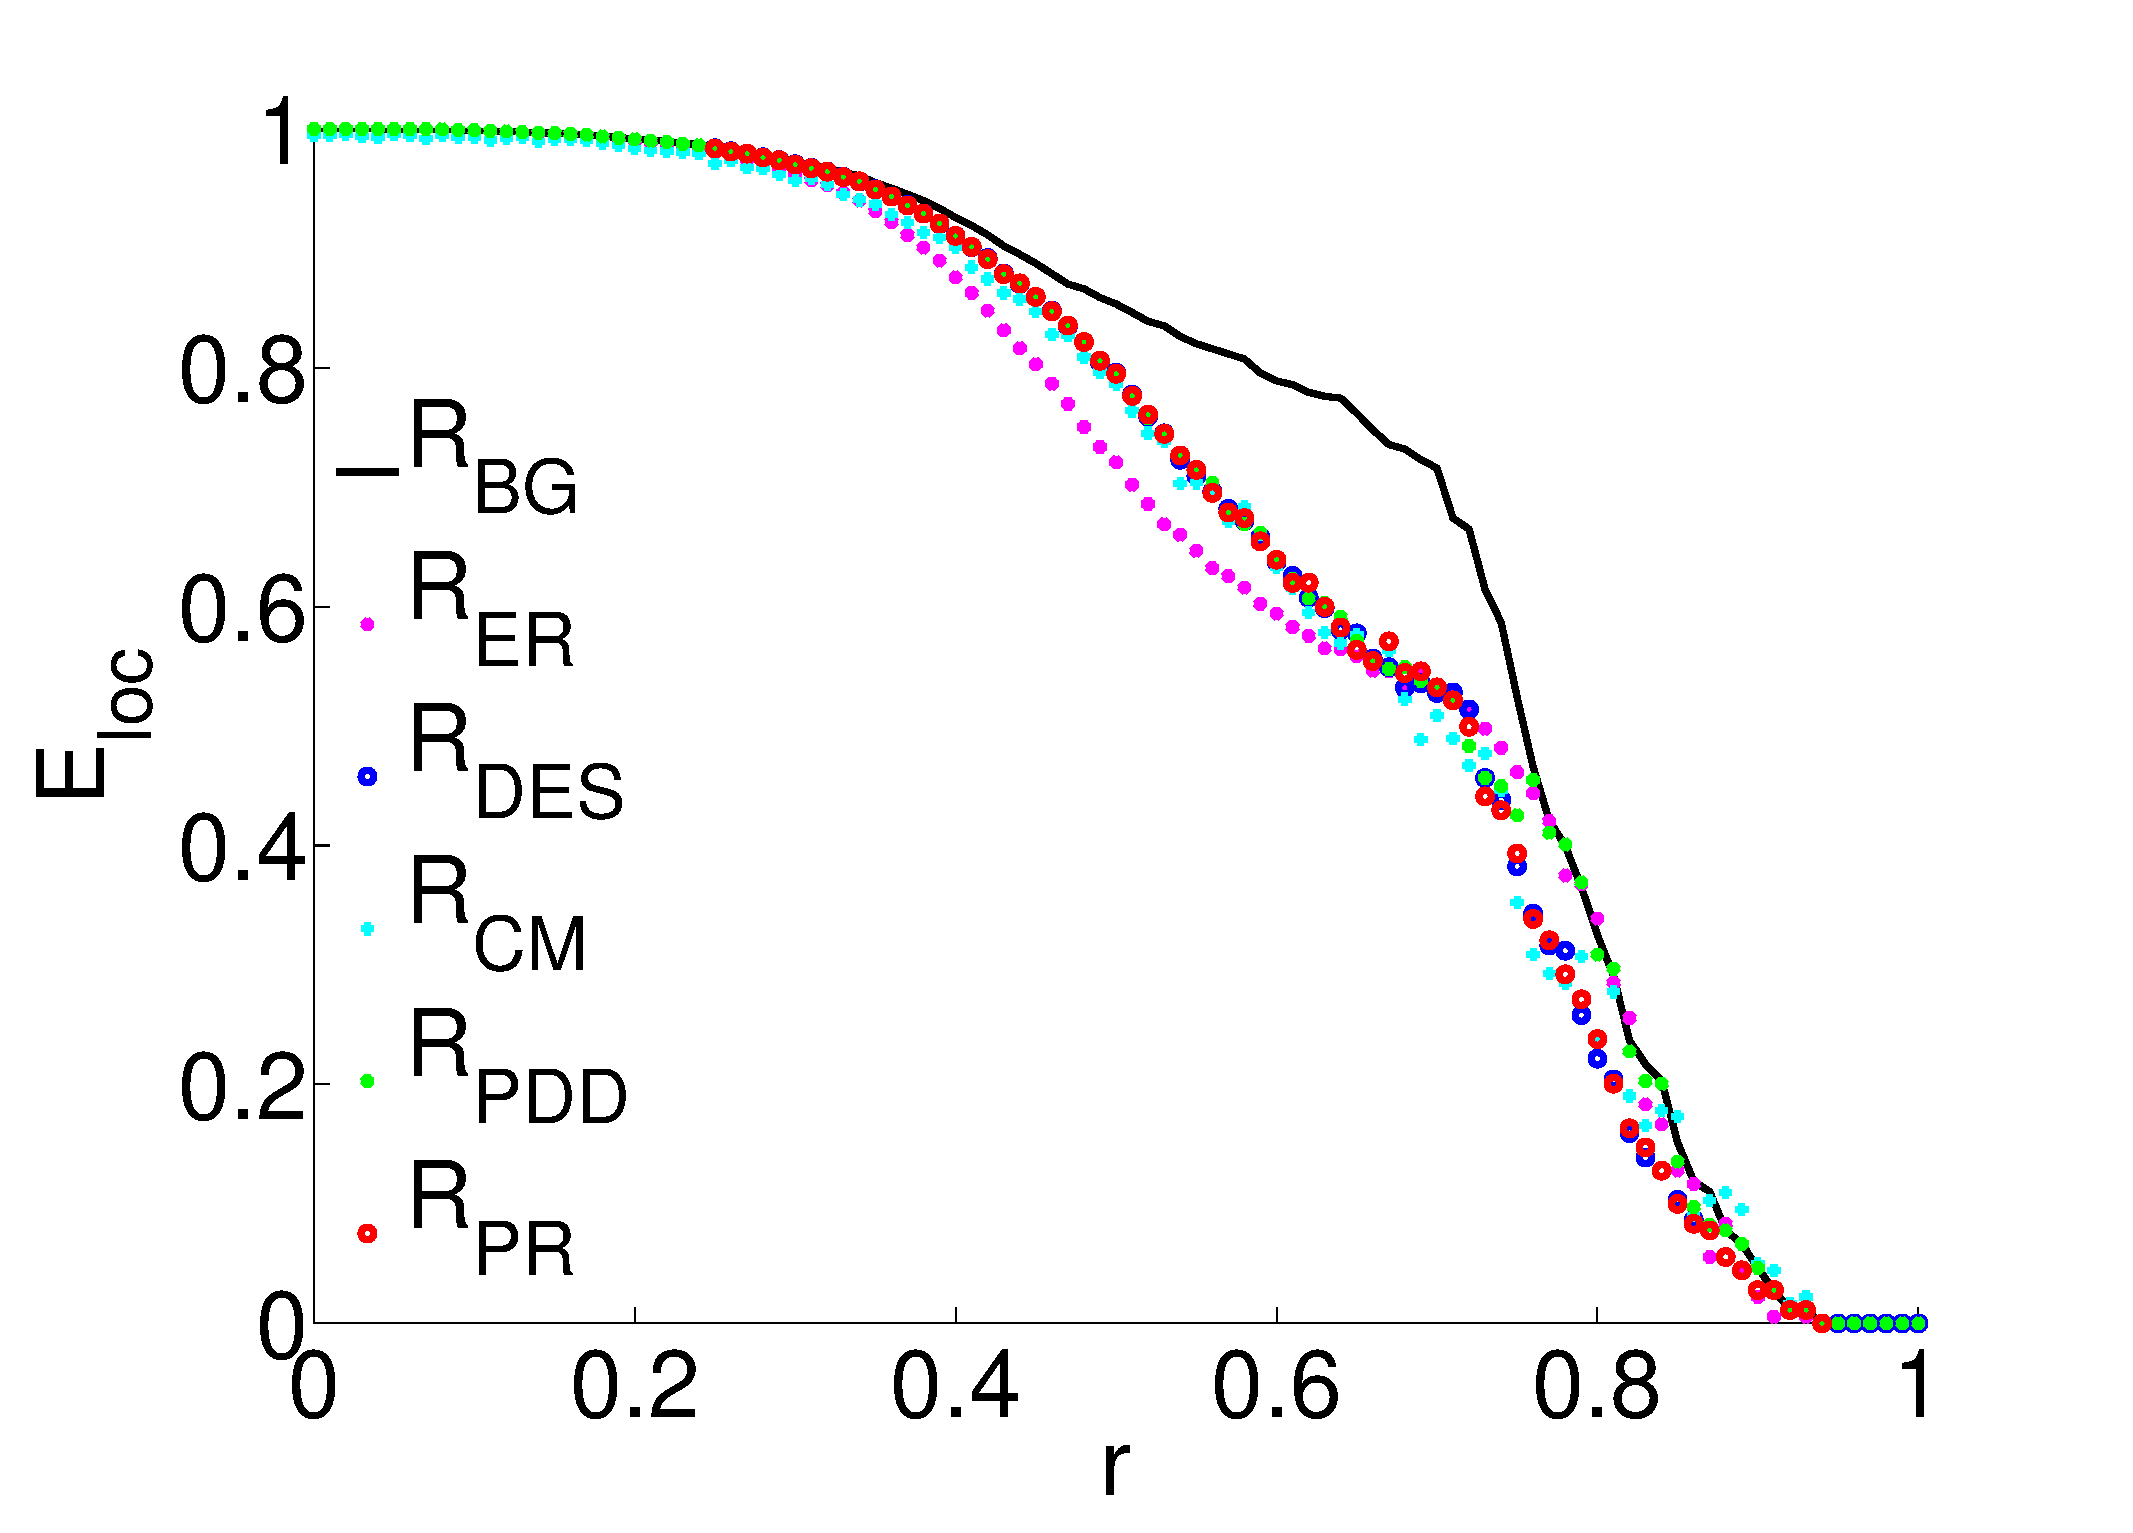
\includegraphics[width=0.49\textwidth]{../reports/MSc_01_report/Local_Efficiency_Average_Fnc.eps}
	 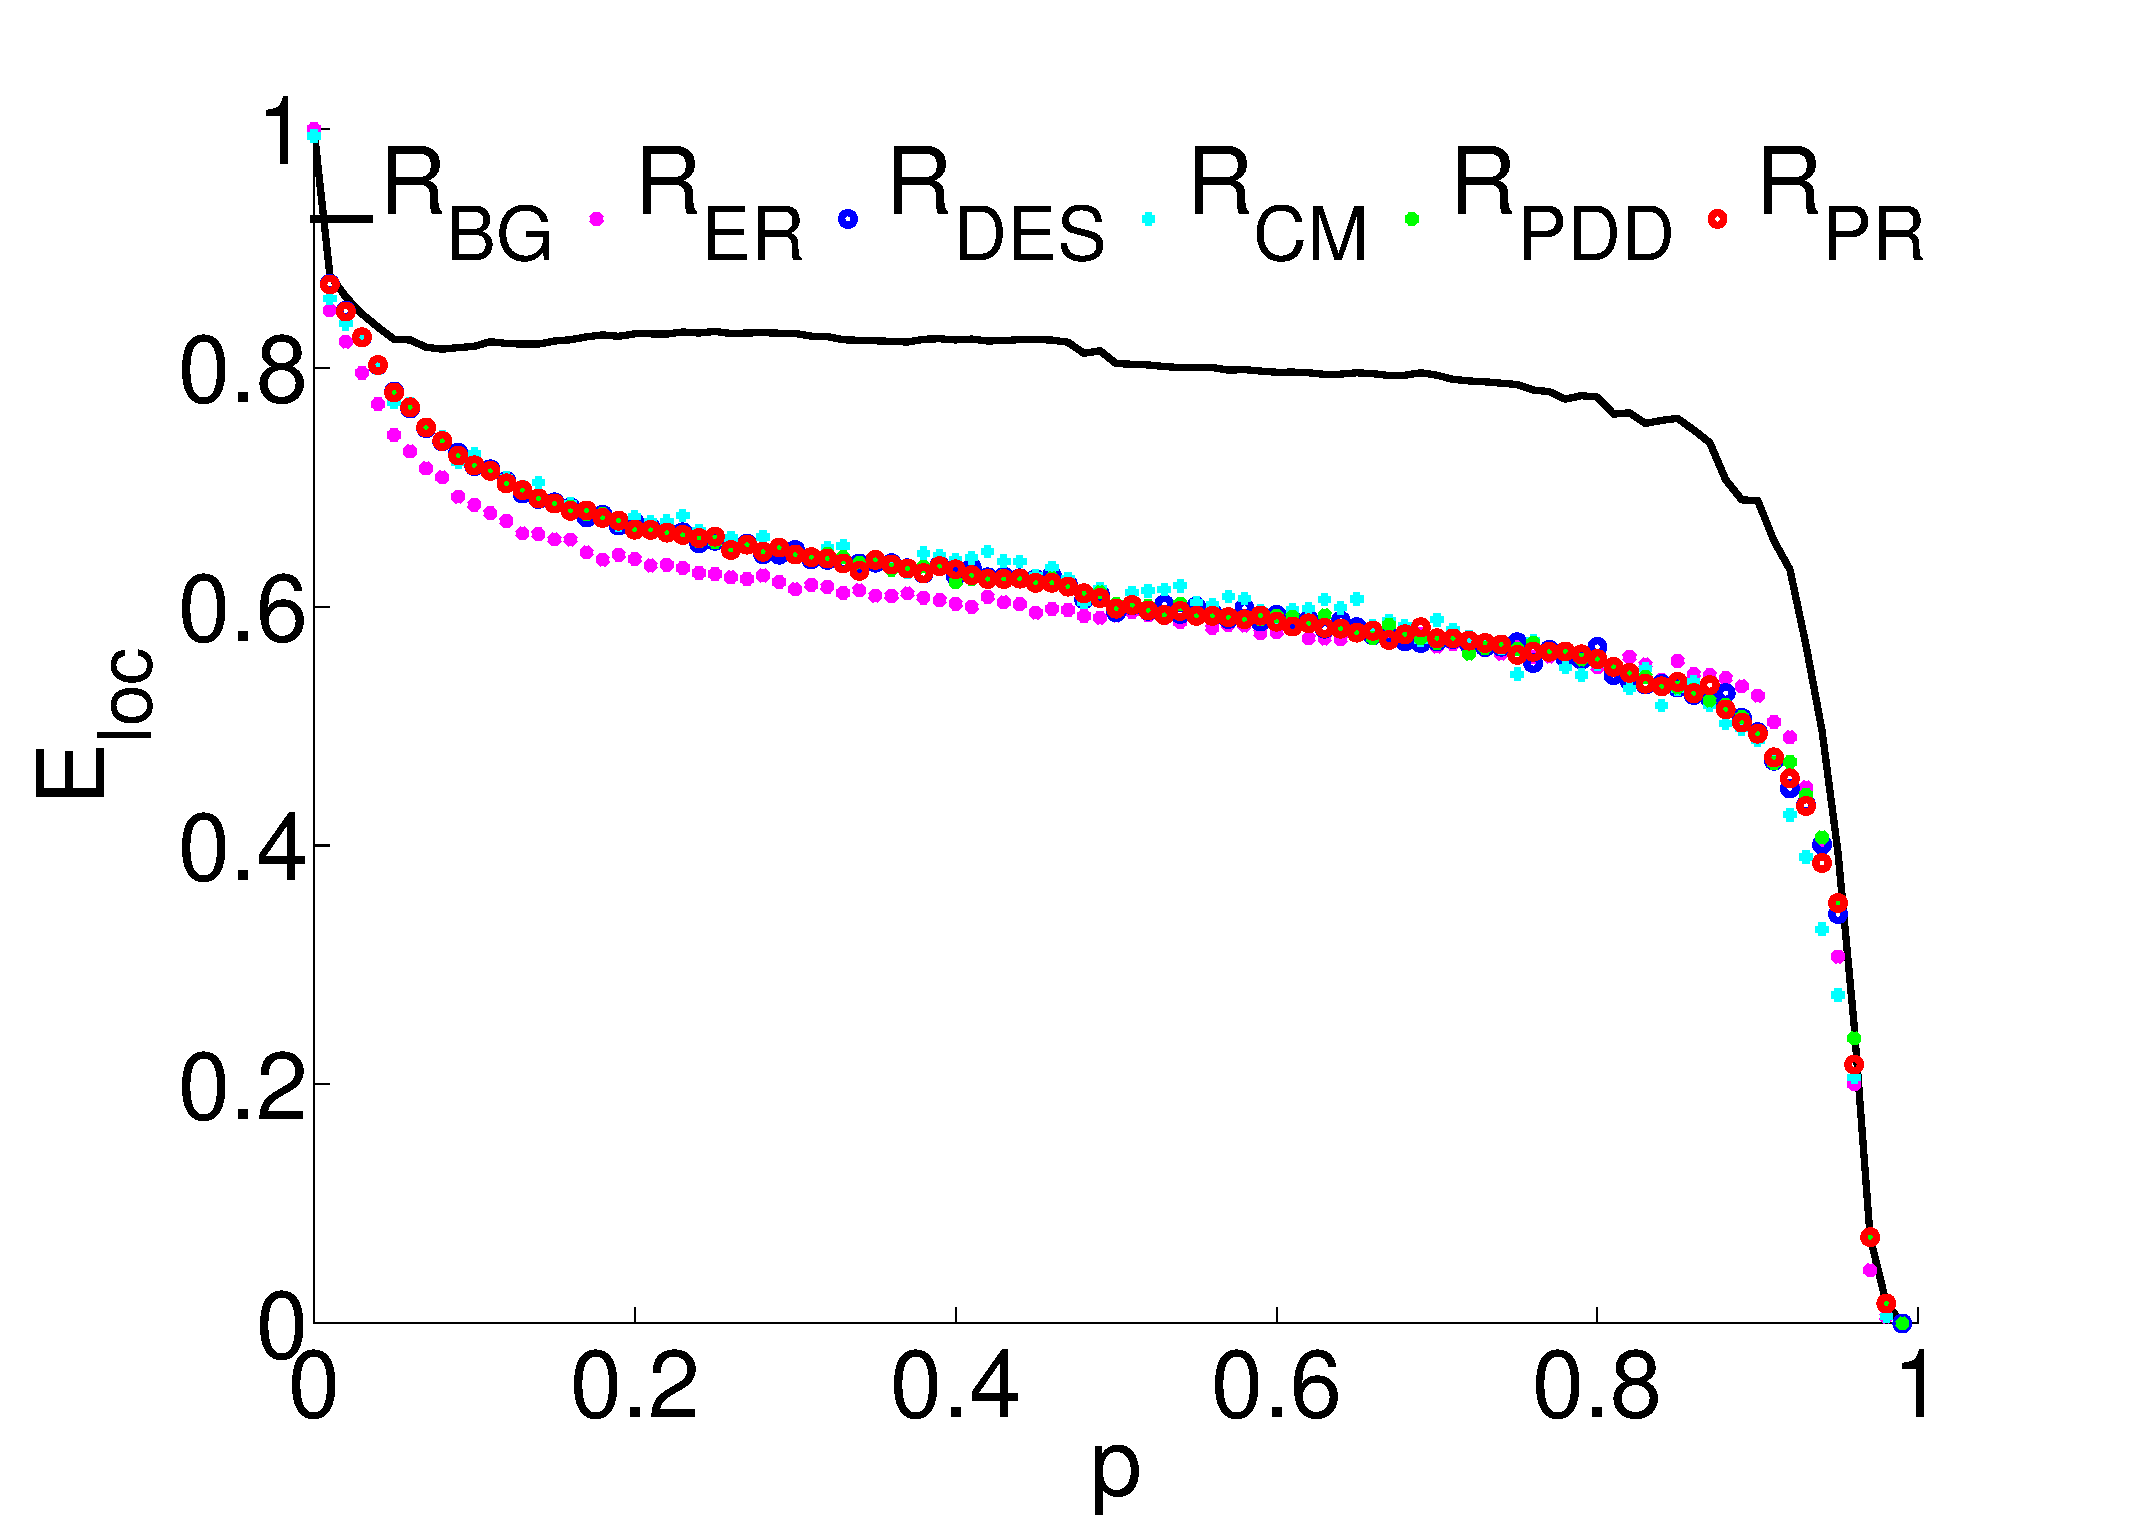
\includegraphics[width=0.49\textwidth]{../reports/MSc_01_report/Local_Efficiency_Average_Stru.eps}
  \caption[Local Efficiency]{Local efficiency of the test networks and random graphs} 
    \label{fig:Local Efficiency}
 	
\end{figure}

Brain graphs based on FCM and ACM tend to have higher $E_{loc}$ than their random graphs. Anatomical connectivity matrix related networks have in general higher $E_{loc}$ compared to the functional connectivity matrix related networks. Local information transmit is more efficient in ACM than in FCM. The graphs with larger $E$ in Figure B.3 exhibit lower $E_{loc}$ in Figure B.4.   


\section{Small Worldness}

A small world network is both highly segregated and integrated, a measure of small worldness $S$ was proposed to capture this effect in a single statistic,

\begin{equation}
S = \frac{C/C_{rand}}{L/L_{rand}}
\end{equation}
 
where $C$ and $C_{rand}$ are clustering coefficients, $L$ and $L_{rand}$ are characteristic path lengths of the original and random network respectively \citep{HUM08}. The random network here is constructed with \textit{Erdos-Renyi} method, which has the same number of nodes and links as the reference graph. 

\begin{equation}
L = \frac{1}{n}\sum\limits_{i \epsilon N} L_i = \frac{1}{n}\sum\limits_{i \epsilon N} \frac{\sum\limits_{j \epsilon N, j \neq i }d_{ij}}{n-1 } 
\end{equation}


\begin{figure}[htbp]
 
  \centering
	 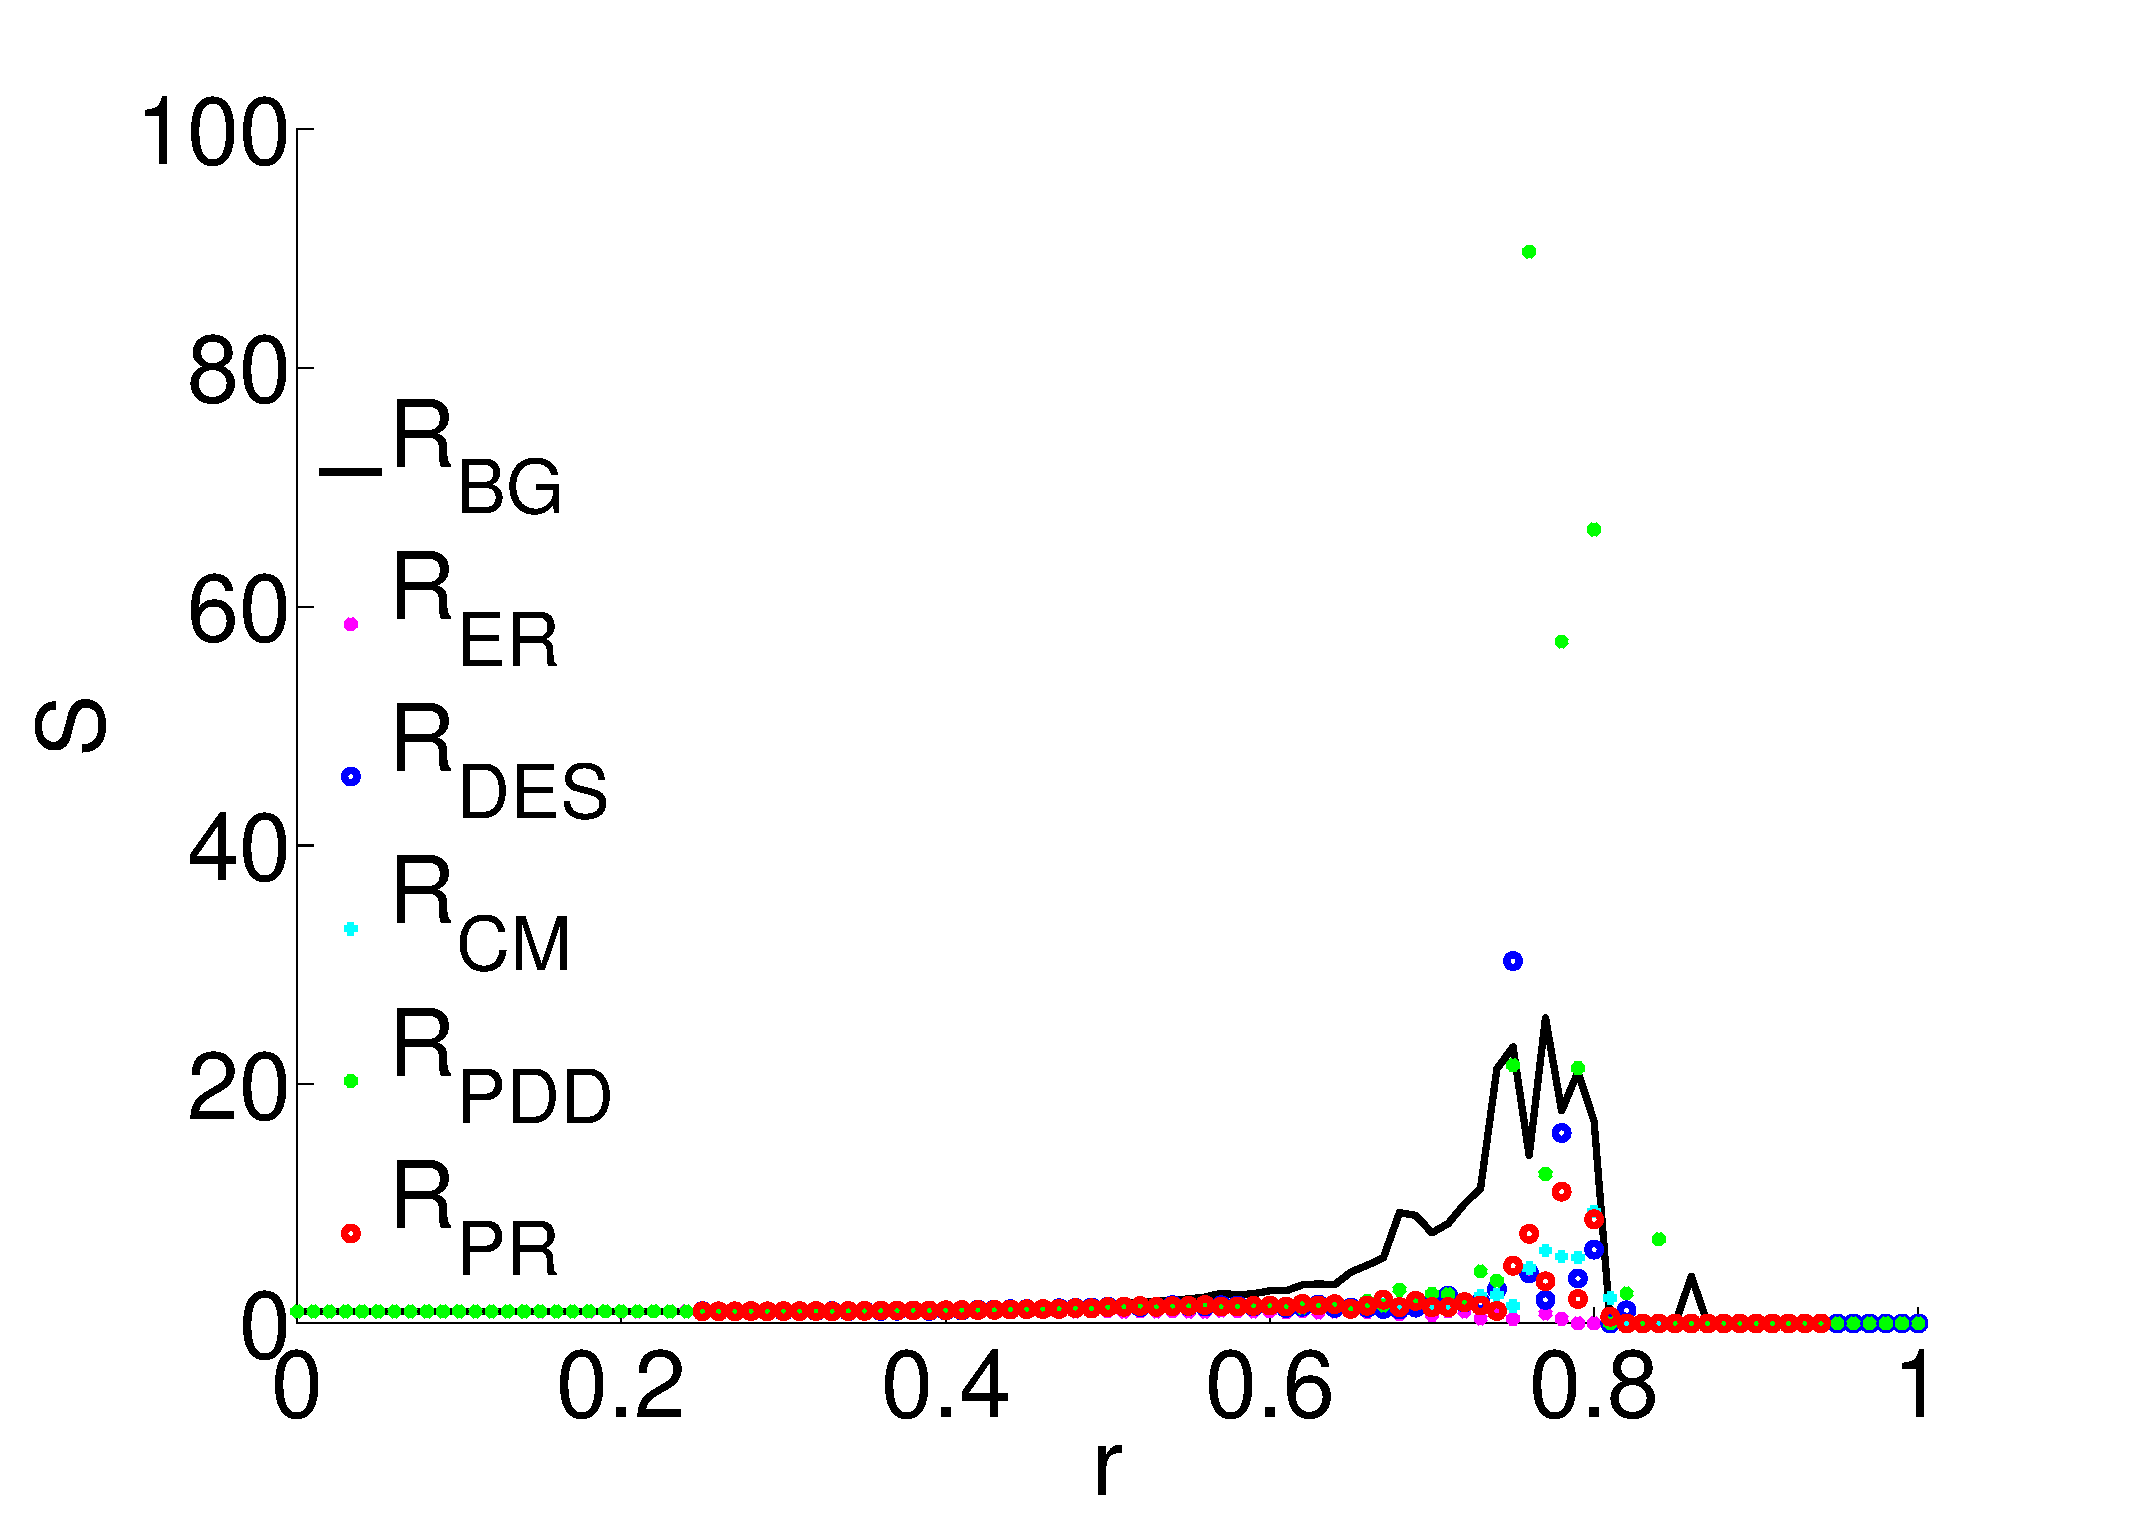
\includegraphics[width=0.49\textwidth]{../reports/MSc_01_report/Small_Worldness_Fnc.eps}
	 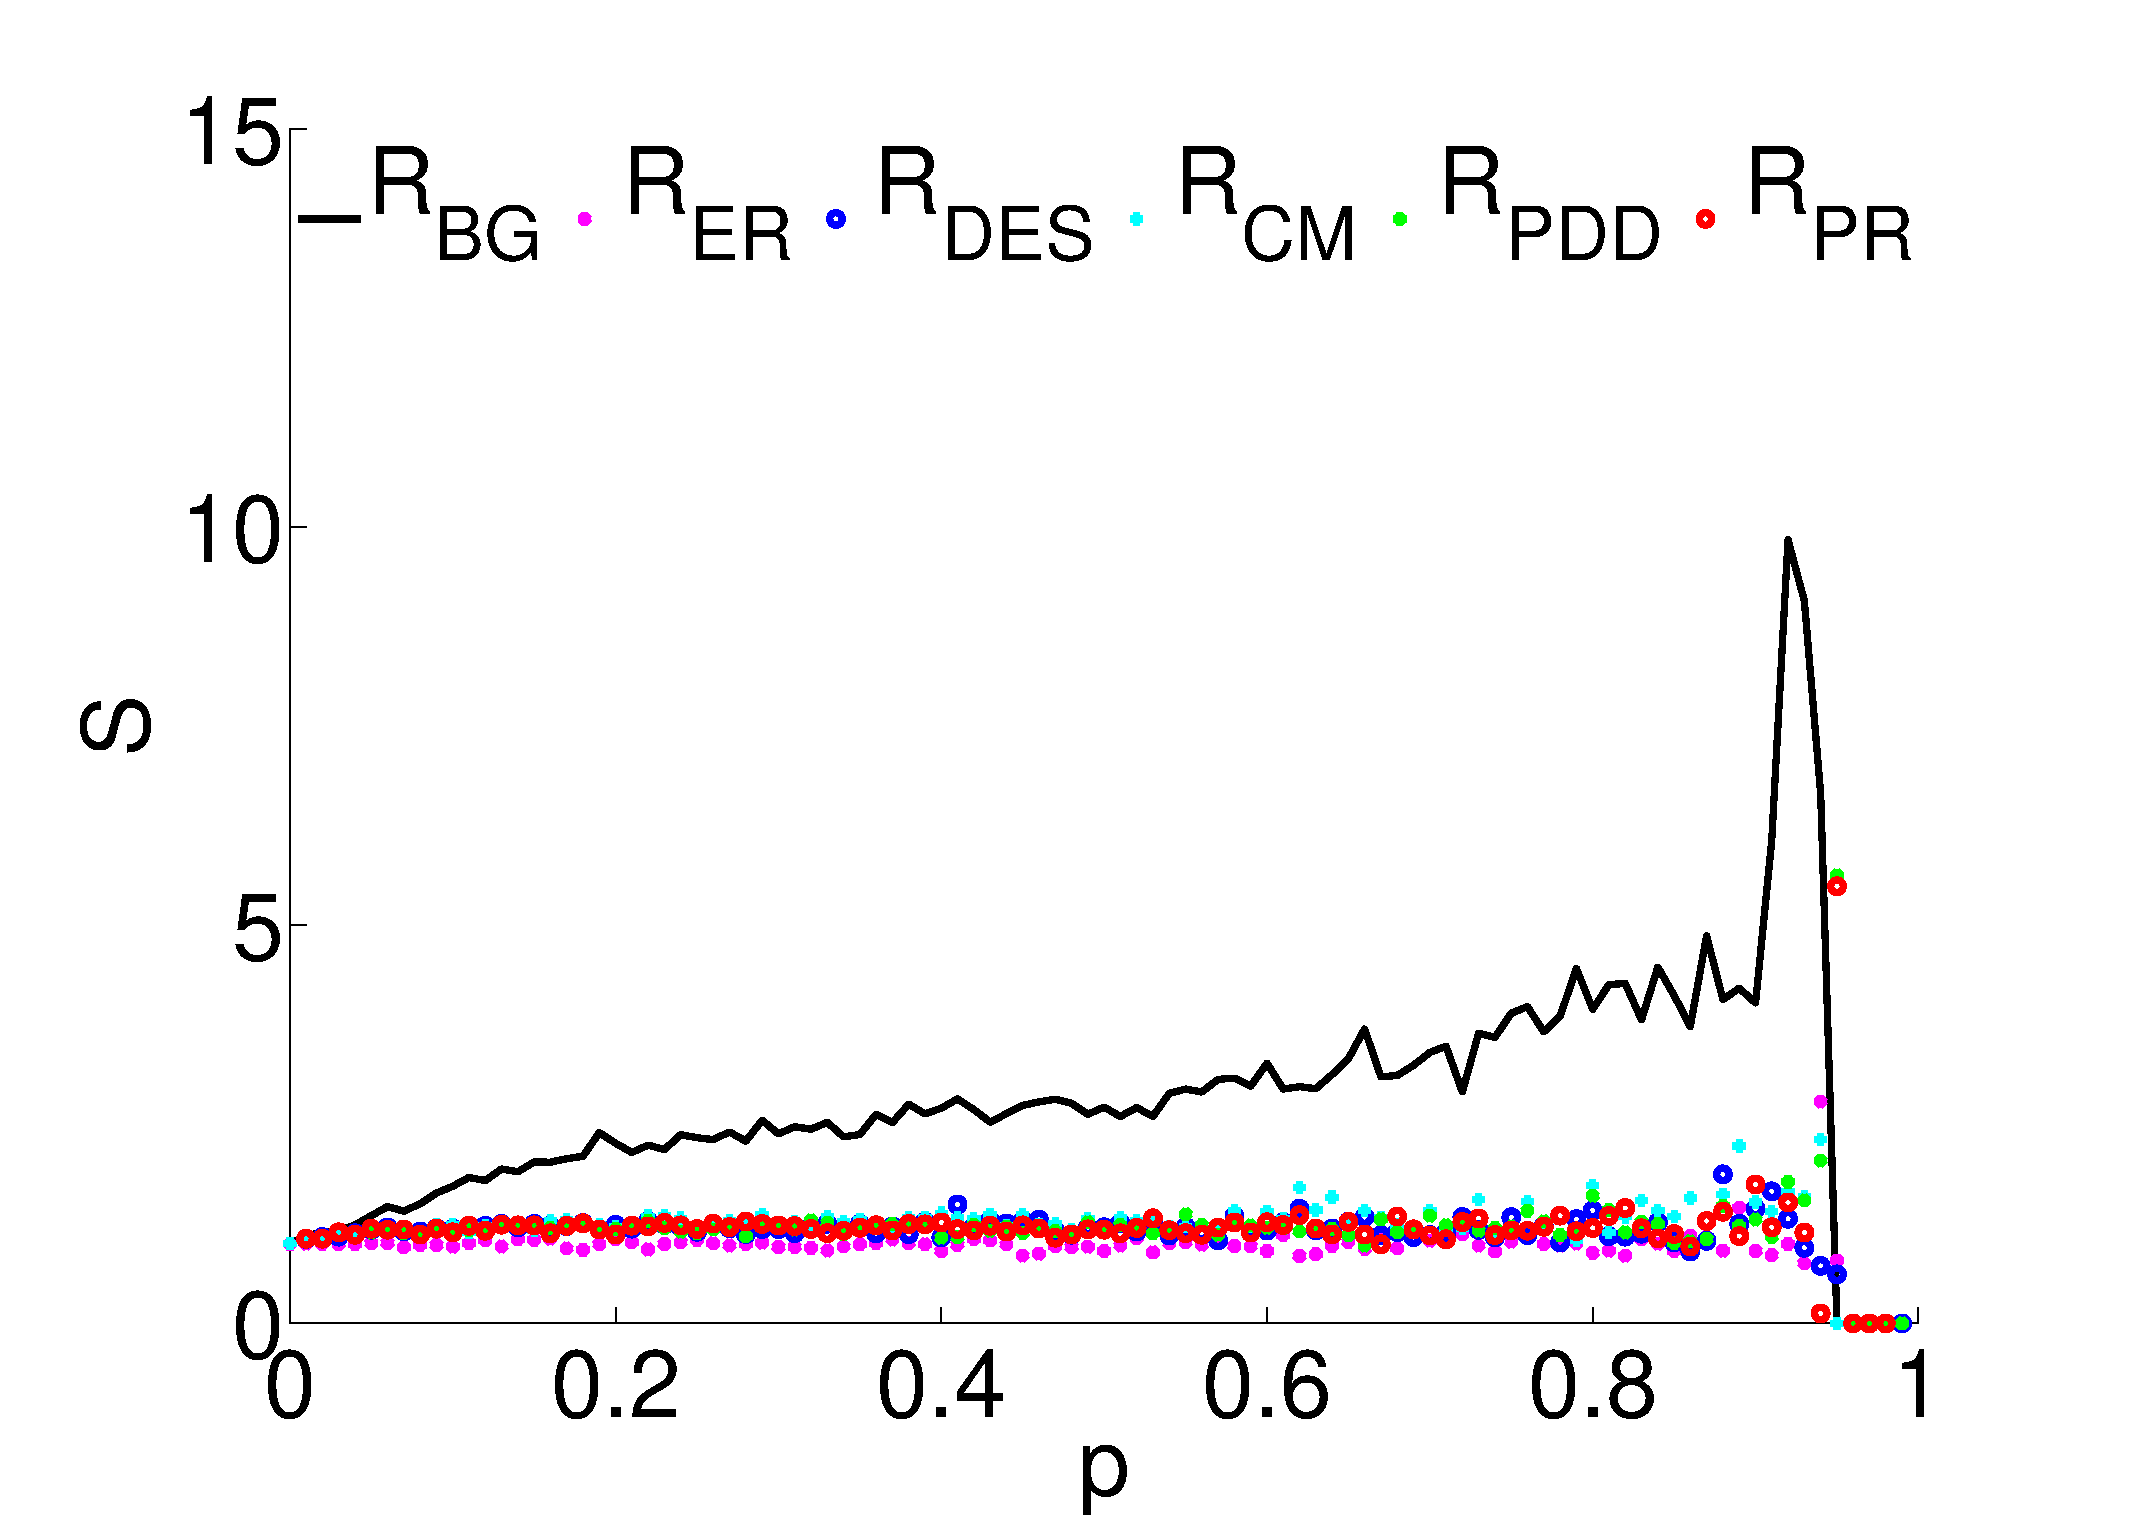
\includegraphics[width=0.49\textwidth]{../reports/MSc_01_report/Small_Worldness_Stru.eps}
  \caption[Small Worldness]{Small worldness of the brain graphs and random graphs.} 
    \label{fig:Small Worldness}
 	
\end{figure}


In Figure B.5, brain graphs have higher $S$ than random graphs for both FCM and ACM. In comparison to other network measurements, $S$ measure makes brain graphs the most distinguishable than random graphs. At some unique $r$ and $p$ values, random graphs $Rd$ (for FCM) and $Rk$ (for ACM) tend to have quite large $S$, however, this does not change the general high $S$ pattern of brain graphs. Random networks seem to be equally segregated and integrated in general, but the real networks behave differently. 



\section{Assortativity}

Assortativity measures the correlation coefficient between the degrees of all nodes on two opposite ends of a link \citep{RUB10}. Assortativity coefficient $A$ of a network, 

\begin{equation}
A = \frac{\dfrac{1}{l} \sum\limits_{(i,j) \in L}  k_i k_j -  \Big ( \dfrac{1}{2L} \sum\limits_{(i,j) \in L}k_i + k_j  \Big )^2}{\dfrac{1}{2L}\sum\limits_{(i,j) \in L} ( k_i^2+  k_j^2) -\Big ( \dfrac{1}{2L} \sum\limits_{(i,j) \in L}k_i + k_j  \Big )^2 }
\end{equation}

where $L$ is number of edges in, $k_i$ is degree of node $i$ \citep{NEW02a}.


\begin{figure}[htbp]
 
  \centering
	 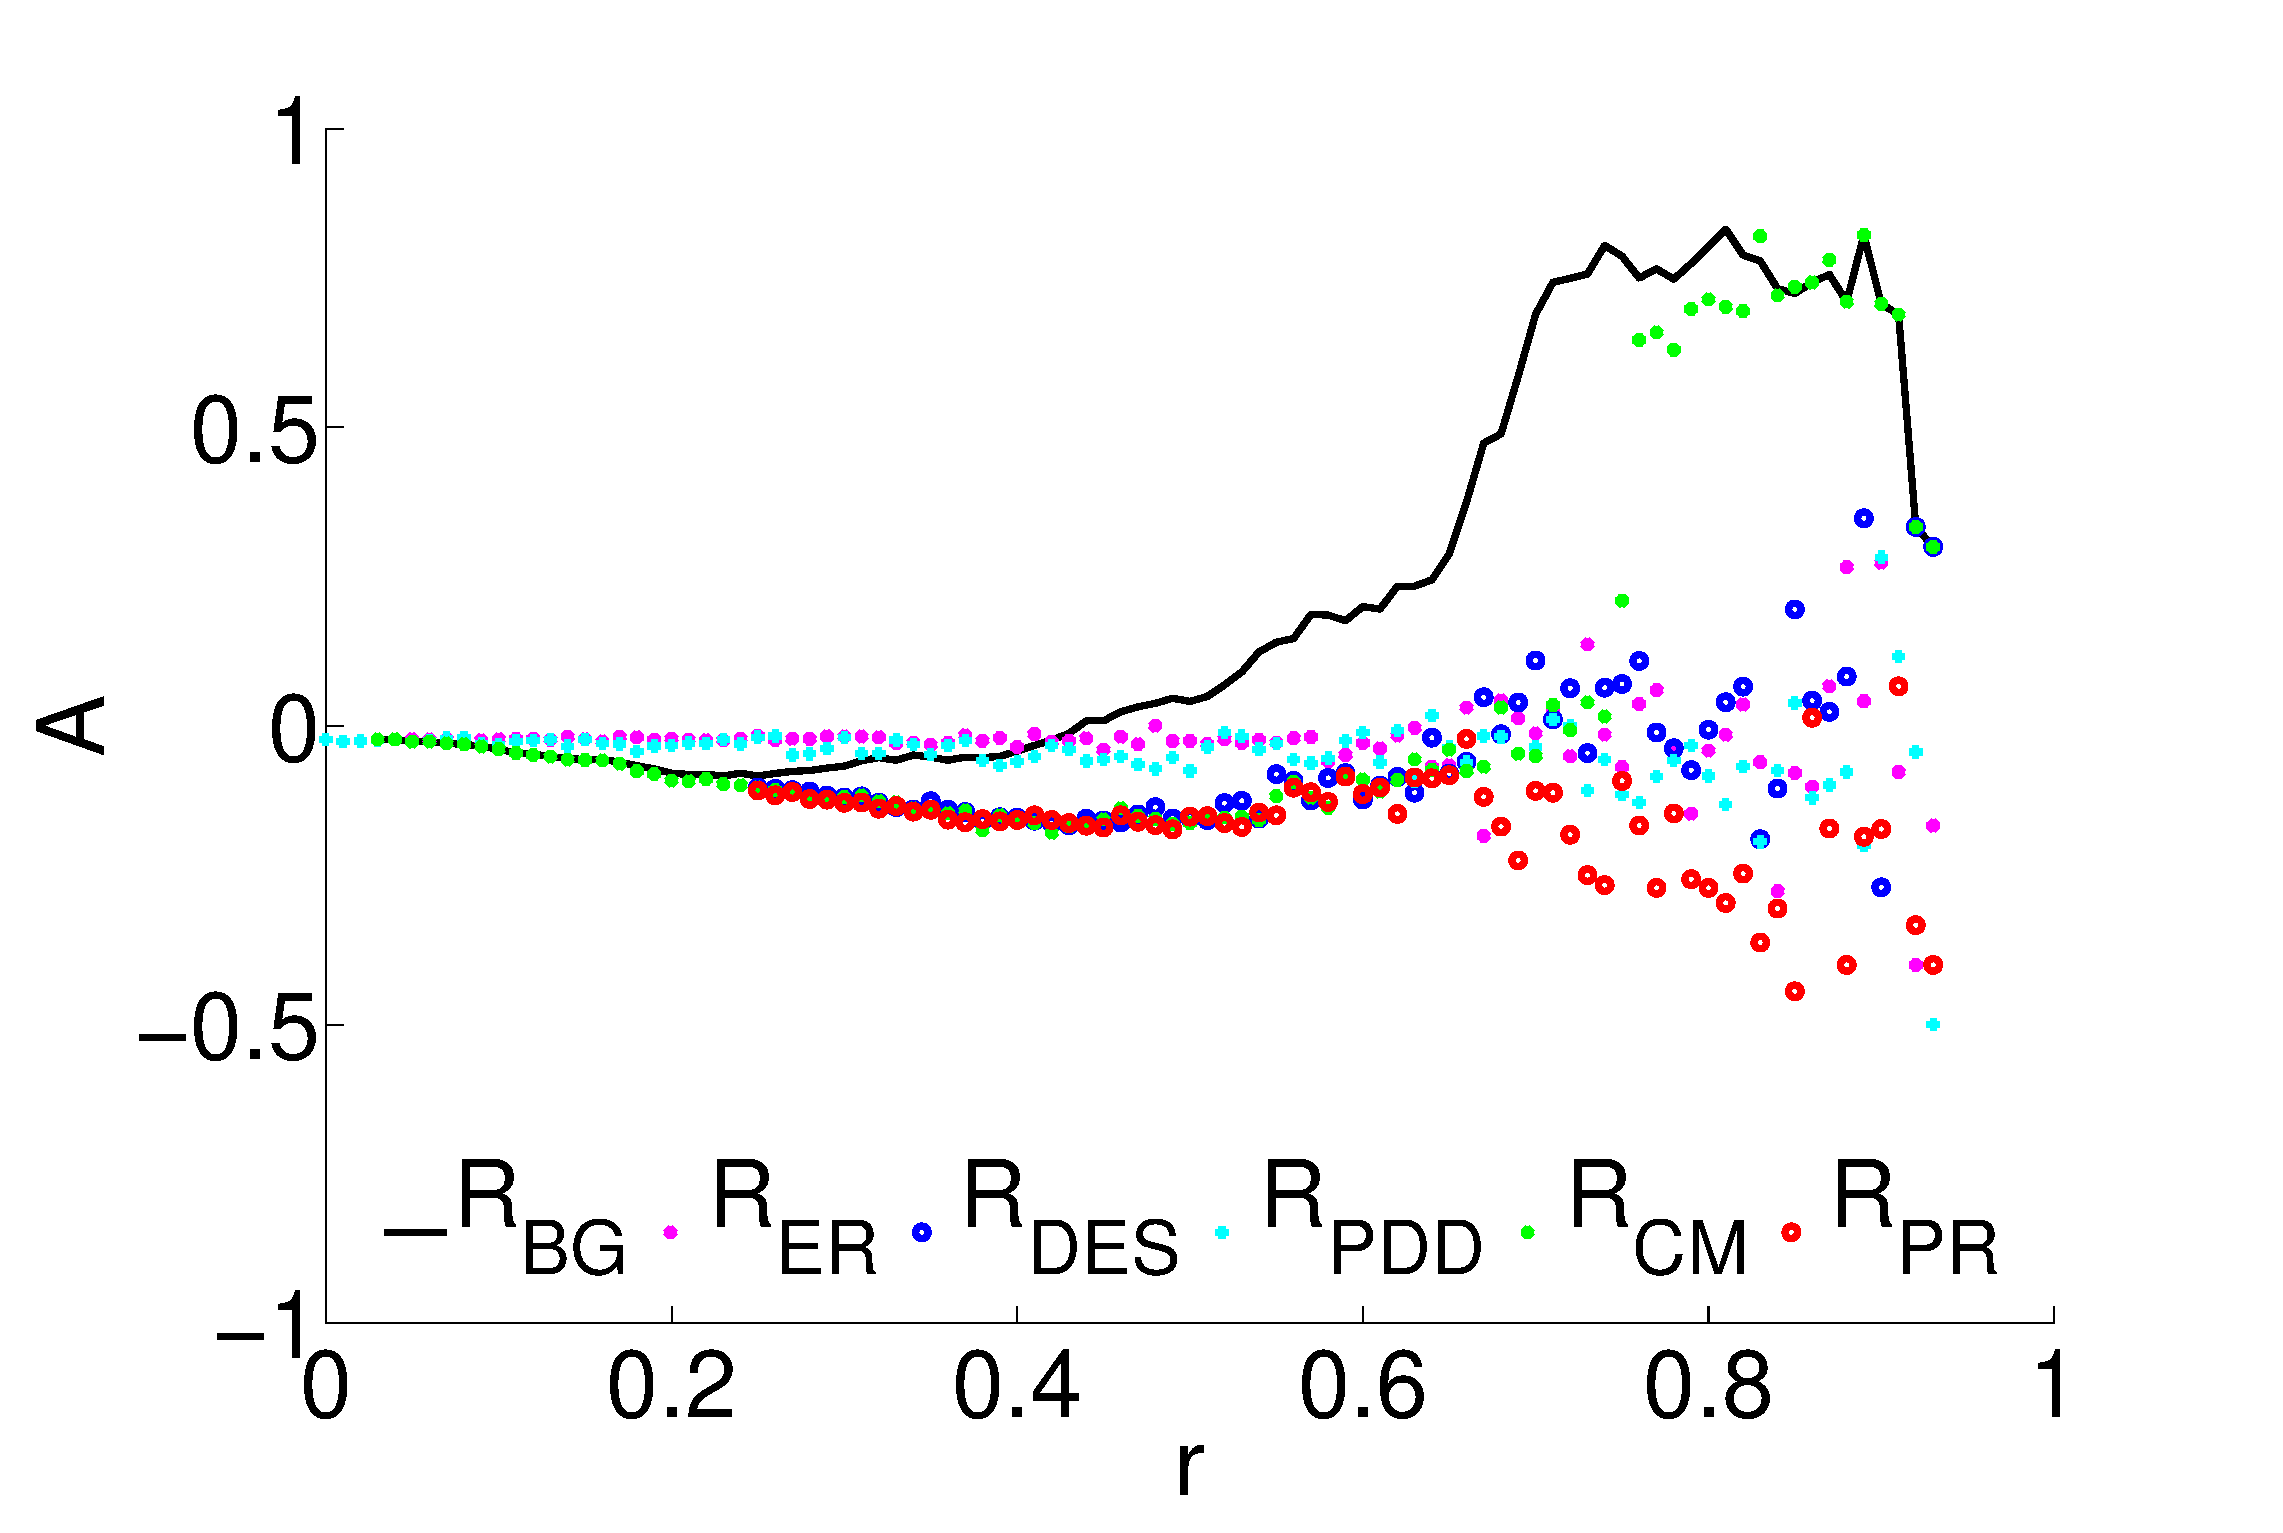
\includegraphics[width=0.49\textwidth]{../reports/MSc_01_report/Assortativity_Fnc.eps}
	 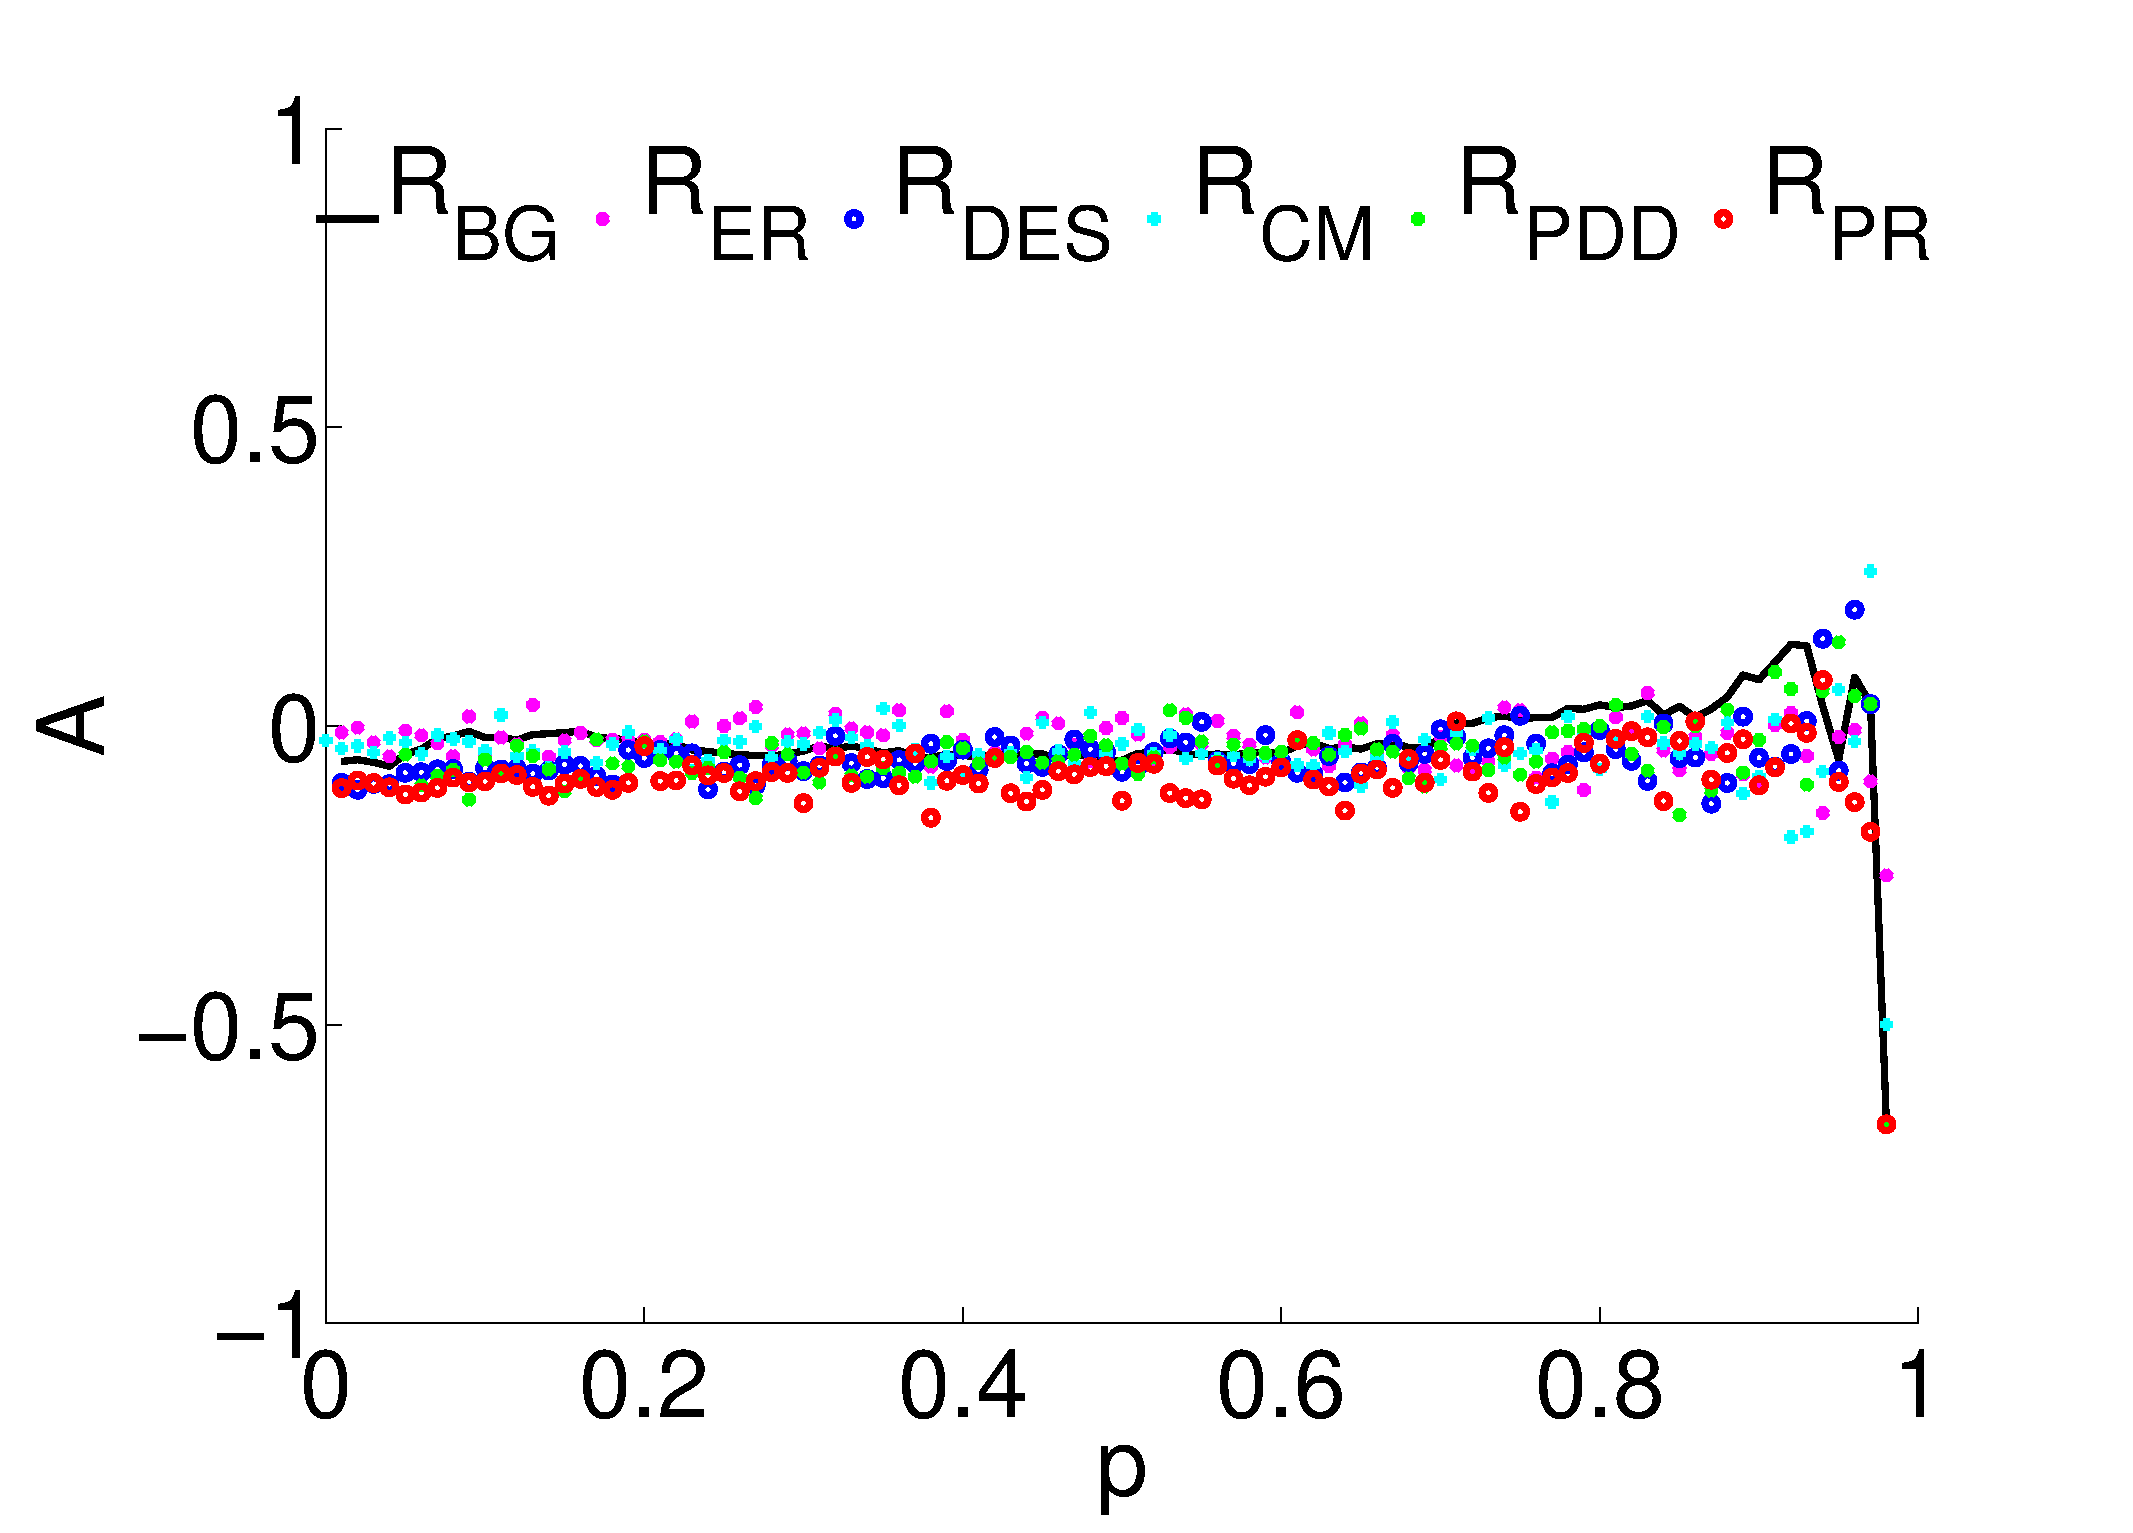
\includegraphics[width=0.49\textwidth]{../reports/MSc_01_report/Assortativity_Stru.eps}
  \caption[Assortativity]{Assortativity coefficients of brain graphs and random graphs} 
    \label{fig:Assortativity}
 	
\end{figure}

Negative assortativity presents a network having widely distributed high-degree hubs \citep{RUB10}. On the other hand, assortativity coefficients close to $1$ indicates a graph having fine correlated degree nodes. $A$ values follow a very similar pattern around 0 for all the graphs based on ACM as seen in Figure B.6. The degrees of nodes seem not to be significantly correlated. However, $A$ of FCM related networks are more diverse. The degrees of nodes are highly correlated in FCM brain graph, particularly at large $r$, whereas random graphs exhibit anti-correlations among node degrees.   

\section{Degree Distribution}
Degree distribution of a network reflects the probability ($P(k)$) of a node to have a given number of degree ($k$). Degree distribution reveals the resilience of a graph. 

\begin{equation}
 P(k) = \sum\limits_{k' \geq k} p(k')
\end{equation}

where $p(k')$ is the probability of a node having degree $k'$ \citep{BAR99a}. 


\begin{figure}[htbp]
 
  \centering
	 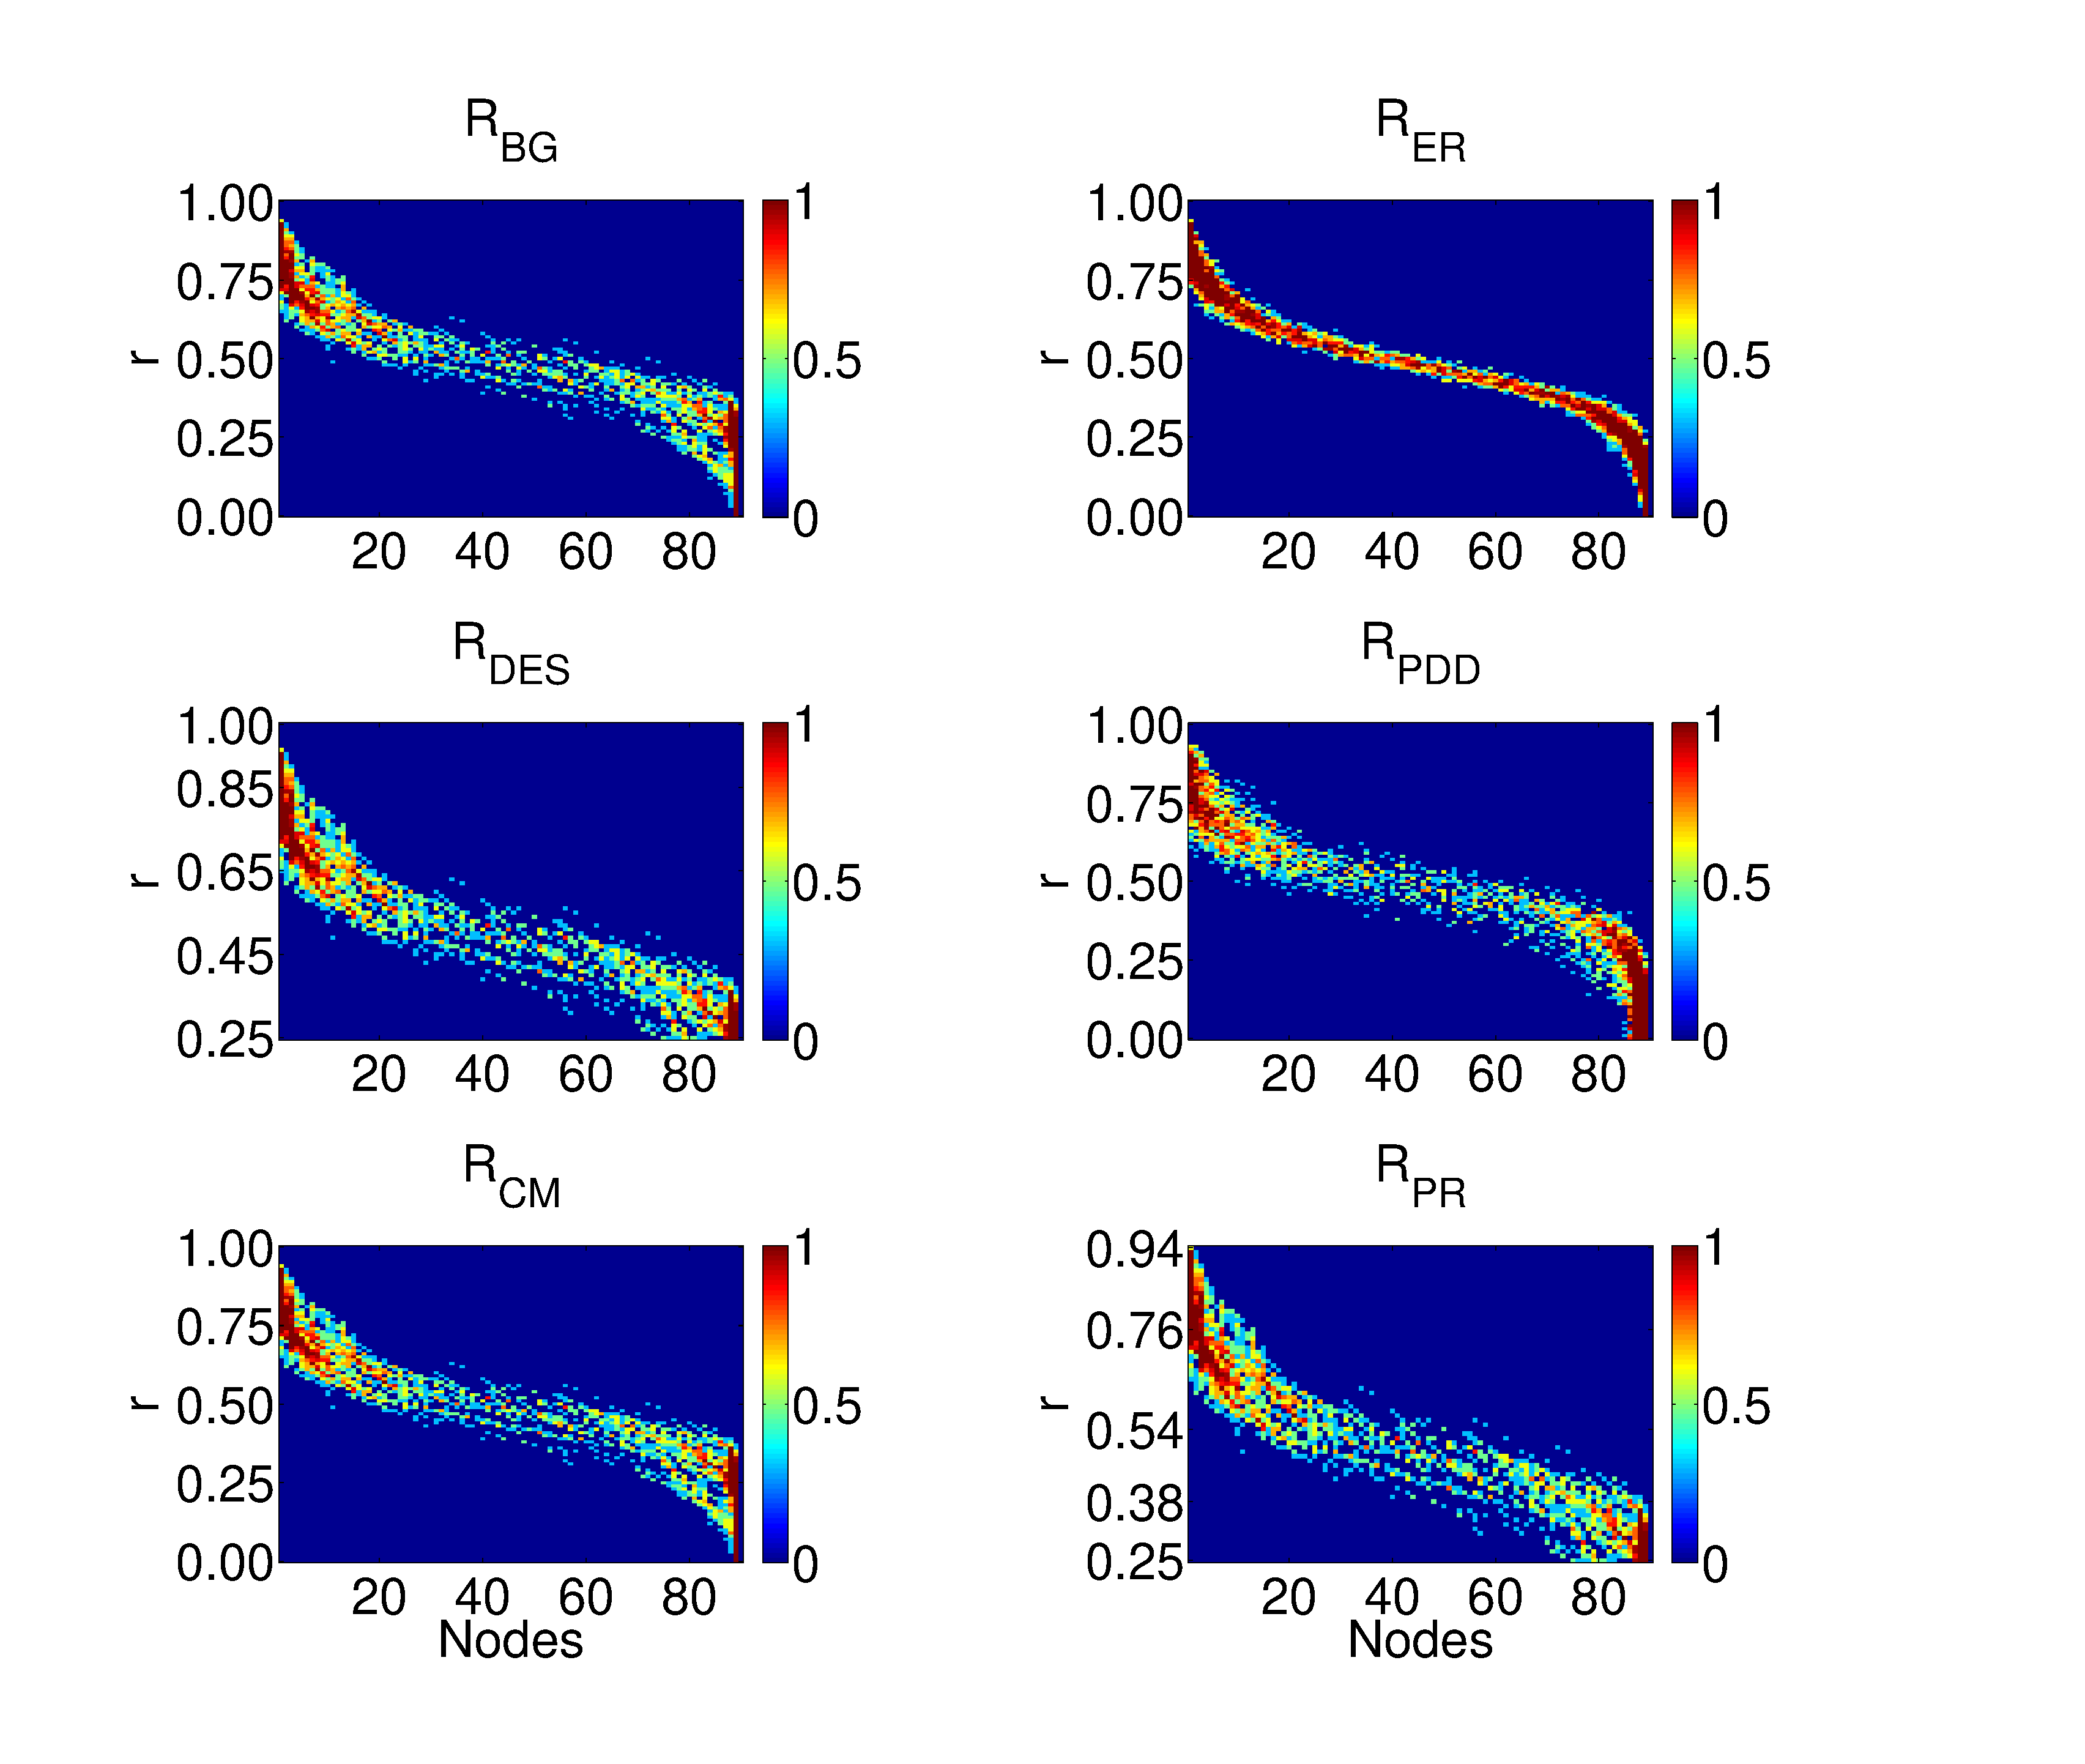
\includegraphics[width=0.8\textwidth, height=110mm]{../reports/MSc_01_report/Degree_Distribution_Fnc.eps}
  \caption[Degree Distribution, FCM]{Heat maps of $P(k)$ of the FCM network. The limits of colorbar are $[log_{10}(10^0), log_{10}(10^1)]$} 
    \label{fig:Degree Distribution, FCM}
 	
\end{figure}



\begin{figure}[htbp]
 
  \centering
	 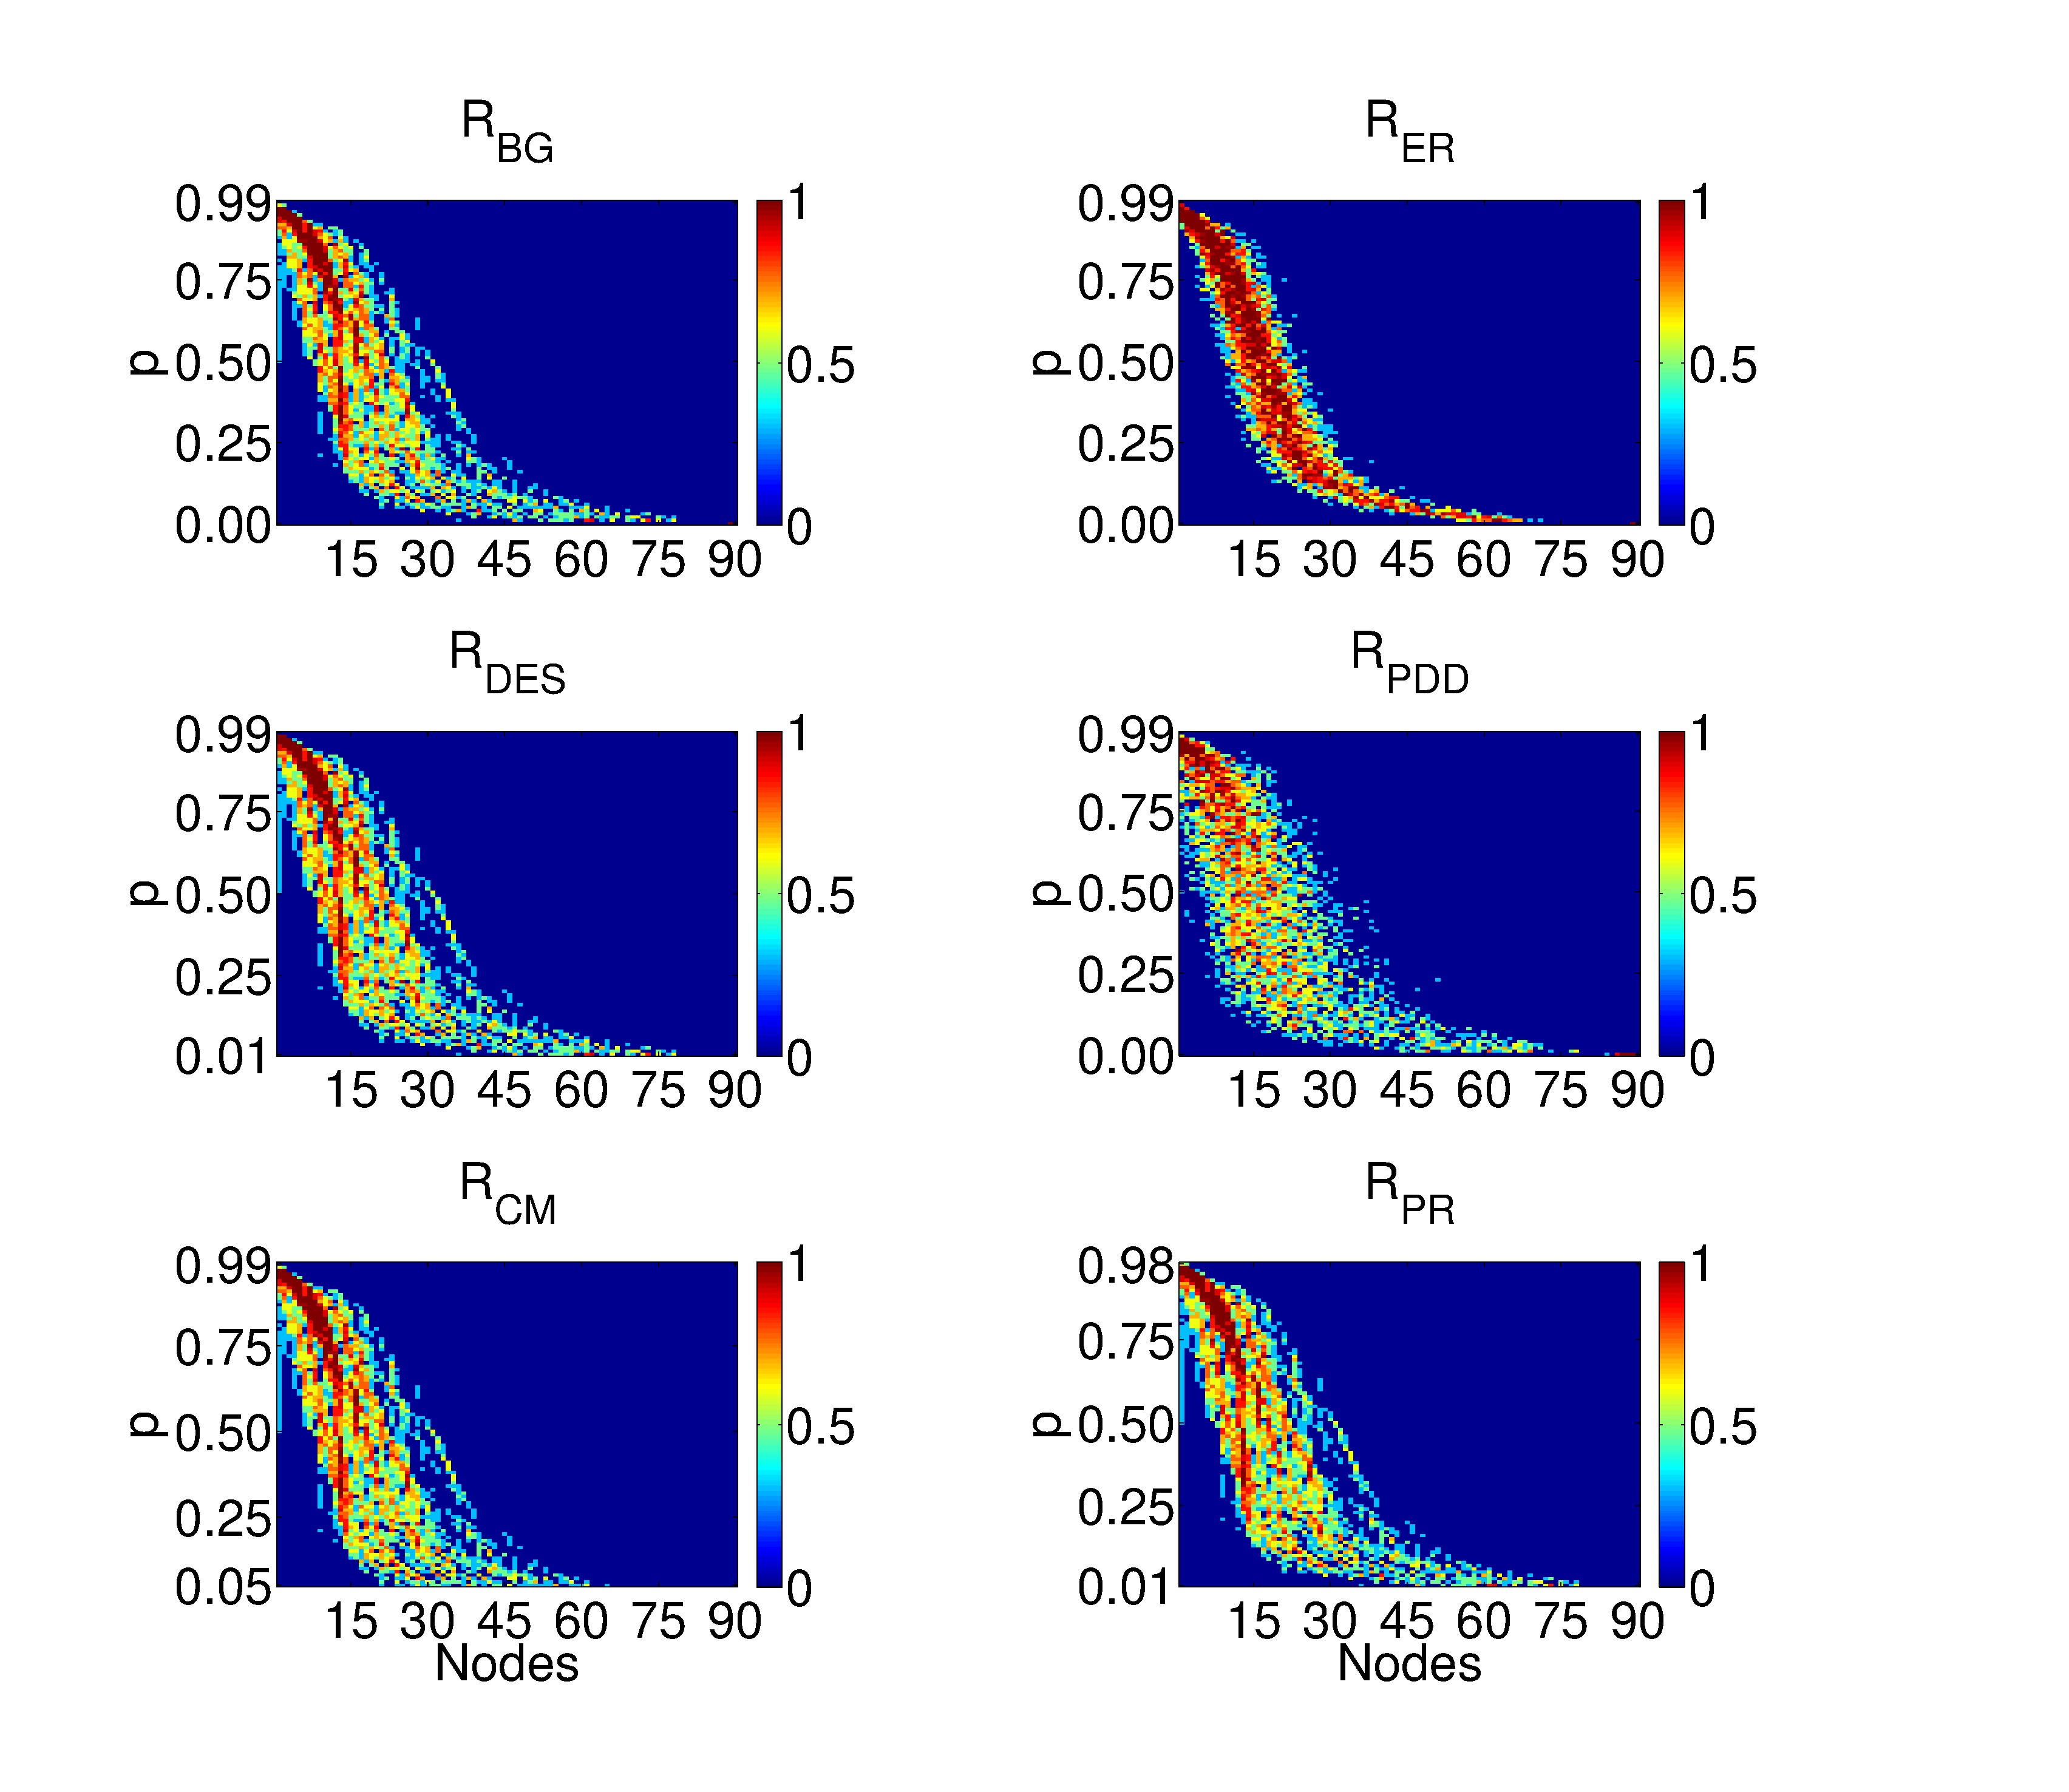
\includegraphics[width=0.8\textwidth, height=110mm]{../reports/MSc_01_report/Degree_Distribution_Stru.eps}
  \caption[Degree Distribution, ACM]{Heat maps of $P(k)$ of the ACM network. The limits of colorbar are $[log_{10}(10^0), log_{10}(10^1)]$} 
    \label{fig:Degree Distribution, ACM}
 	
\end{figure}



